\documentclass[11pt,a4paper]{article}

\usepackage[english]{babel}
\usepackage[T1]{fontenc}
\usepackage[utf8]{inputenc}

% Math essentials
\usepackage{amsmath, amssymb}
\usepackage{bm}

% Units and hyperlinks
\usepackage{siunitx}
\sisetup{per-mode=symbol}

\usepackage{natbib}
\usepackage{graphicx}
\usepackage{lmodern}
\usepackage{caption}
\usepackage{subcaption}
\usepackage{float}
\usepackage{url}
\usepackage{titlepic}
\usepackage{listings}
\usepackage{nameref}
\usepackage{xcolor}
\usepackage{array}
\setlength{\marginparwidth}{2cm}
\usepackage{todonotes}
\usepackage{datetime}
\usepackage{parskip}
\usepackage{hyperref}

% ------- Macros defined in this document -------
\newcommand{\vect}[1]{\bm{#1}}       % bold italic vectors
\newcommand{\mat}[1]{\mathbf{#1}}    % bold upright matrices
\newcommand{\trans}{\mathsf{T}}      % transpose, use as ^{\trans}

\newcommand{\skewsym}[1]{\left[#1\right]_\times}

\newcommand{\SkewFrom}[3]{%
    \begin{bmatrix}
        \phantom{-}0   & -#3            & \phantom{-}#2  \\
        \phantom{-}#3  & \phantom{-}0   & -#1 \\
        -#2            & \phantom{-}#1  & \phantom{-}0
        \end{bmatrix}
}

\newcommand{\frameR}{\mathcal{R}}
\newcommand{\ejeXR}{X_{\frameR}}
\newcommand{\ejeYR}{Y_{\frameR}}

\newcommand{\frameB}{\mathcal{B}}
\newcommand{\ejeXB}{X_{\frameB}}
\newcommand{\ejeYB}{Y_{\frameB}}

\newcommand{\frameBi}{\mathcal{B}_i}
\newcommand{\ejeXBi}{X_{\frameBi}}
\newcommand{\ejeYBi}{Y_{\frameBi}}

\newcommand{\frameBZero}{\mathcal{B}_0}
\newcommand{\frameBNMinusOne}{\mathcal{B}_{N-1}}

\newcommand{\frameW}{\mathcal{W}}
\newcommand{\ejeXW}{X_{\frameW}}
\newcommand{\ejeYW}{Y_{\frameW}}

\newcommand{\frameWi}{\mathcal{W}_i}
\newcommand{\ejeXWi}{X_{\frameWi}}
\newcommand{\ejeYWi}{Y_{\frameWi}}

\title{Ground Robotics Kinematics: A Generalized Framework for Forward and Inverse Kinematics of Wheeled Terrestrial Robots}
\author{Juan Francisco Rascón Crespo}
\date{\today}

\setcounter{secnumdepth}{2}
\setcounter{tocdepth}{2}

\begin{document}
\maketitle

\begin{abstract}
    This document presents a rigorous analytical development of the forward and inverse kinematics for wheeled terrestrial robots. Starting from the definition of an invariant base coordinate system for each wheel, a system of matrix equations is formulated that relates the individual velocities to the chassis's state of motion. Given that platforms with multiple wheels typically generate overdetermined systems, their optimal resolution is addressed using the least squares method and the Moore-Penrose pseudoinverse. The text places a fundamental emphasis on software implementation and numerical stability, comprehensively justifying the use of Singular Value Decomposition (SVD) to bypass algebraic instabilities. Furthermore, the condition number (\(\kappa\)) analysis is introduced as a critical diagnostic tool to distinguish between the computational robustness of the algorithm and the physical viability of the mechanical design. Finally, this generalized theoretical framework is applied to the kinematic formulation and resolution of various standard topologies in mobile robotics, ranging from differential drive and Ackermann steering systems to omnidirectional platforms with Mecanum wheels and \textit{swerve drive} configurations.
\end{abstract}

\section{Motion constraints imposed by the wheels}

In a terrestrial robot, the wheels impose motion constraints. In conventional wheels, whether steerable or non-steerable, as the wheel rotates about its axis of rotation, it moves following a straight path in a specific direction called the \textbf{rolling direction}. In non-steerable conventional wheels, the rolling direction is fixed, always pointing in the same direction, since the wheel cannot change its orientation relative to the chassis. In steerable conventional wheels, the wheel first orients itself toward the desired rolling direction (pivoting on its vertical axis) and then rotates about its axis of rotation to move in that direction. Both steerable and non-steerable conventional wheels cannot move in the direction perpendicular to the rolling direction, which is the direction of their rotation axis. In other words, the lateral velocity of the wheel is zero, which is known as the \textbf{no-lateral-slip constraint}.

Conversely, in omnidirectional and Mecanum/Swedish wheels, due to the presence of free-spinning rollers on their periphery, the rolling direction of the main wheel, although fixed and unchanging over time, does not necessarily have to coincide with the actual direction of the wheel's movement on the ground. The passive rotation of the rollers allows the wheel to have a non-zero lateral velocity (in a direction perpendicular to the rolling direction; \textit{i.e.}, the direction of the wheel's axis of rotation), eliminating the no-lateral-slip constraint.

These constraints can be expressed mathematically as equations that relate the linear and angular velocity of the wheel to the robot's velocity. These equations are fundamental for the design of controllers and motion planners for terrestrial robots, as they determine how the robot can move in its environment. By stacking these constraints for each wheel, the forward and inverse kinematics equations can be derived for different terrestrial robot configurations, such as differential drive robots, omnidirectional wheeled robots, and steerable active wheeled robots (swerve drive), among others.

Figure \ref{fig:wheel-placement} shows the 2D positioning of a wheel relative to the robot's coordinate system (CS), \(\frameR\). The term \(\alpha\) represents the angle formed by the \(\ejeXR\) axis and the wheel's position vector, \(\vect{d}\), and due to how the wheel is \textit{initially} positioned, it is also the angle formed by the \(\ejeXR\) axis and the \(\ejeYW\) axis. The \(\ejeXW\) axis is perpendicular to the \(\ejeYW\) axis and its orientation with respect to the \(\ejeXR\) axis is \(\psi = \alpha - \frac{\pi}{2}\). The magnitude of the vector \(\vect{d}\) is the distance between the robot's CS and the wheel's CS, \(\left|\bm{d}\right| = d\).

\begin{equation}
    \vect{d} = \begin{bmatrix} d\cos\alpha \\ d\sin\alpha \\ 0 \end{bmatrix}
\end{equation}

\begin{figure}[H]
    \centering
    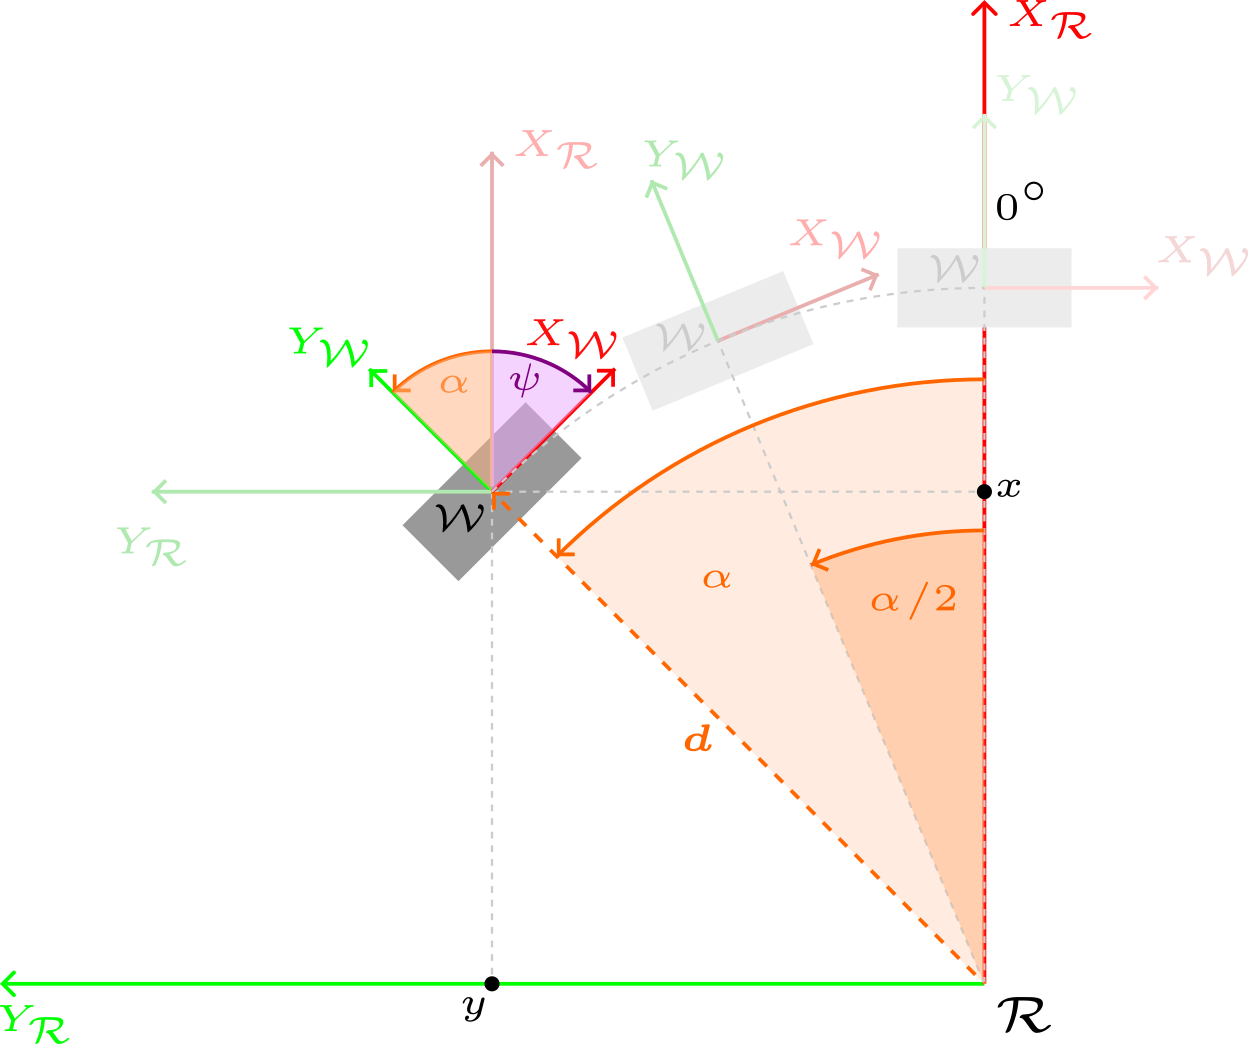
\includegraphics[width=1.0\linewidth]{images/wheel_placement.png}
    \caption{2D positioning of a wheel relative to the robot's CS, \(\frameR\).}
    \label{fig:wheel-placement}
\end{figure}

Next, an angle \(\beta\) is considered, which allows the wheel to be oriented in the desired manner with respect to the robot's CS, \(\frameR\) (Figure \ref{fig:wheel-orientation}), giving rise to the \textbf{wheel's base CS}, \(\frameB\). The CS \(\frameB\) maintains a constant position and orientation over time with respect to the CS \(\frameR\) and is \textit{conveniently suitable} for defining the wheel's orientation during the vehicle's movement and applying the motion constraints. The final orientation of the wheel is given by the angle \(\psi\), formed between the \(\ejeXR\) axis and the \(\ejeXB\) axis.

\[
    \psi = \alpha + \beta - \frac{\pi}{2}
\]

And, to simplify the notation, the symbol \(\phi\) is introduced as:

\[
    \phi = \alpha + \beta, \quad \psi = \phi - \frac{\pi}{2}
\]

\begin{figure}[H]
    \centering
    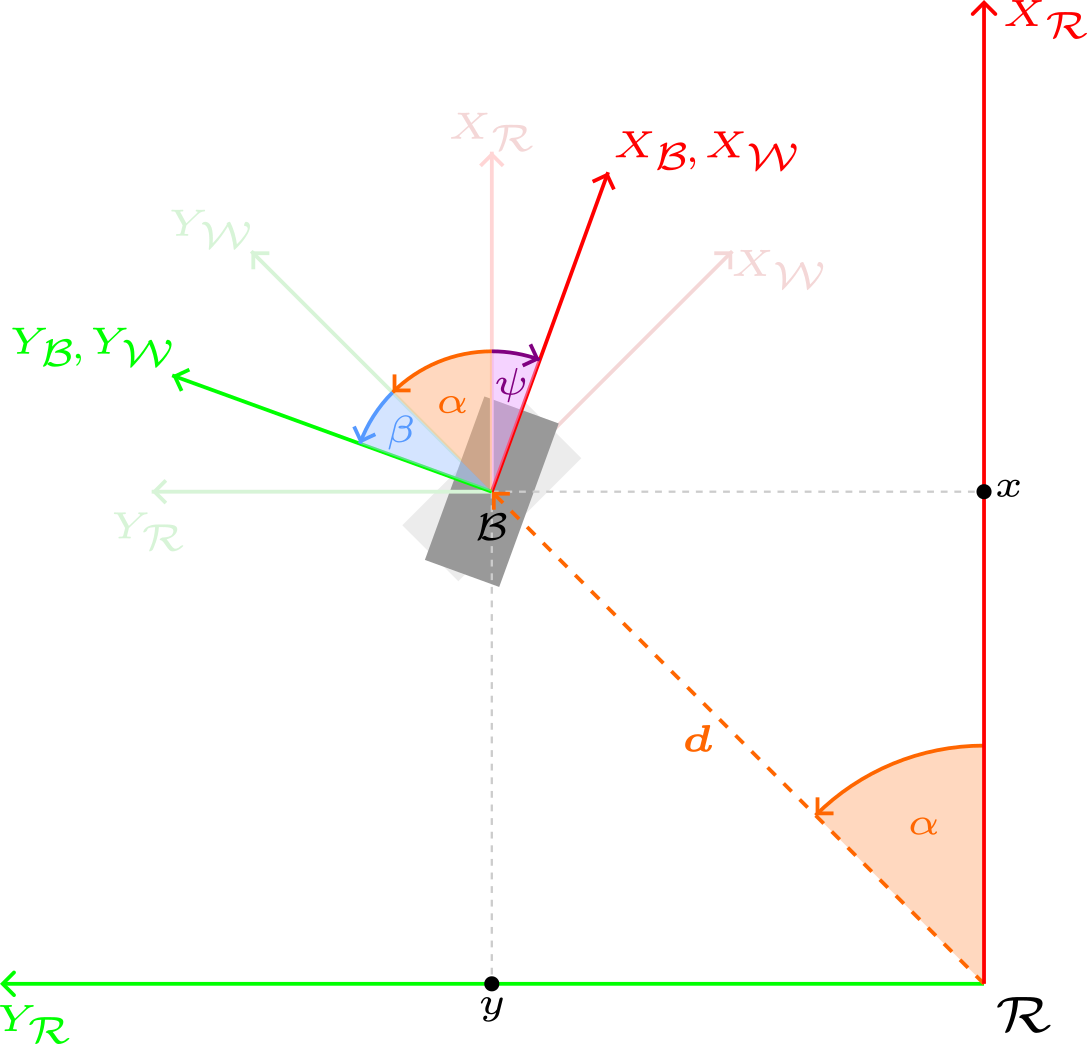
\includegraphics[width=1.0\linewidth]{images/wheel_orientation.png}
    \caption{Orientation of the wheel in the direction of interest, through the angle \(\beta\).}
    \label{fig:wheel-orientation}
\end{figure}

In non-steerable conventional wheels, the \(\ejeXB\) axis and the X axis fixed to the wheel, \(\ejeXW\), which indicates the wheel's rolling direction, coincide all the time. Just for the sake of completeness, it is worth mentioning that in this type of wheels, the \(\ejeYB\) axis and the Y axis fixed to the wheel, \(\ejeYW\), which indicates the direction of its rotation axis, obviously also coincide all the time. In steerable wheels, the CS fixed to the wheel, \(\frameW\), changes its orientation (angle \(\theta\)) with respect to the CS \(\frameB\); that is, only when \(\theta=0\) do both CSs coincide. See Figure \ref{fig:rolling-direction}.

\begin{figure}[H]
    \centering
    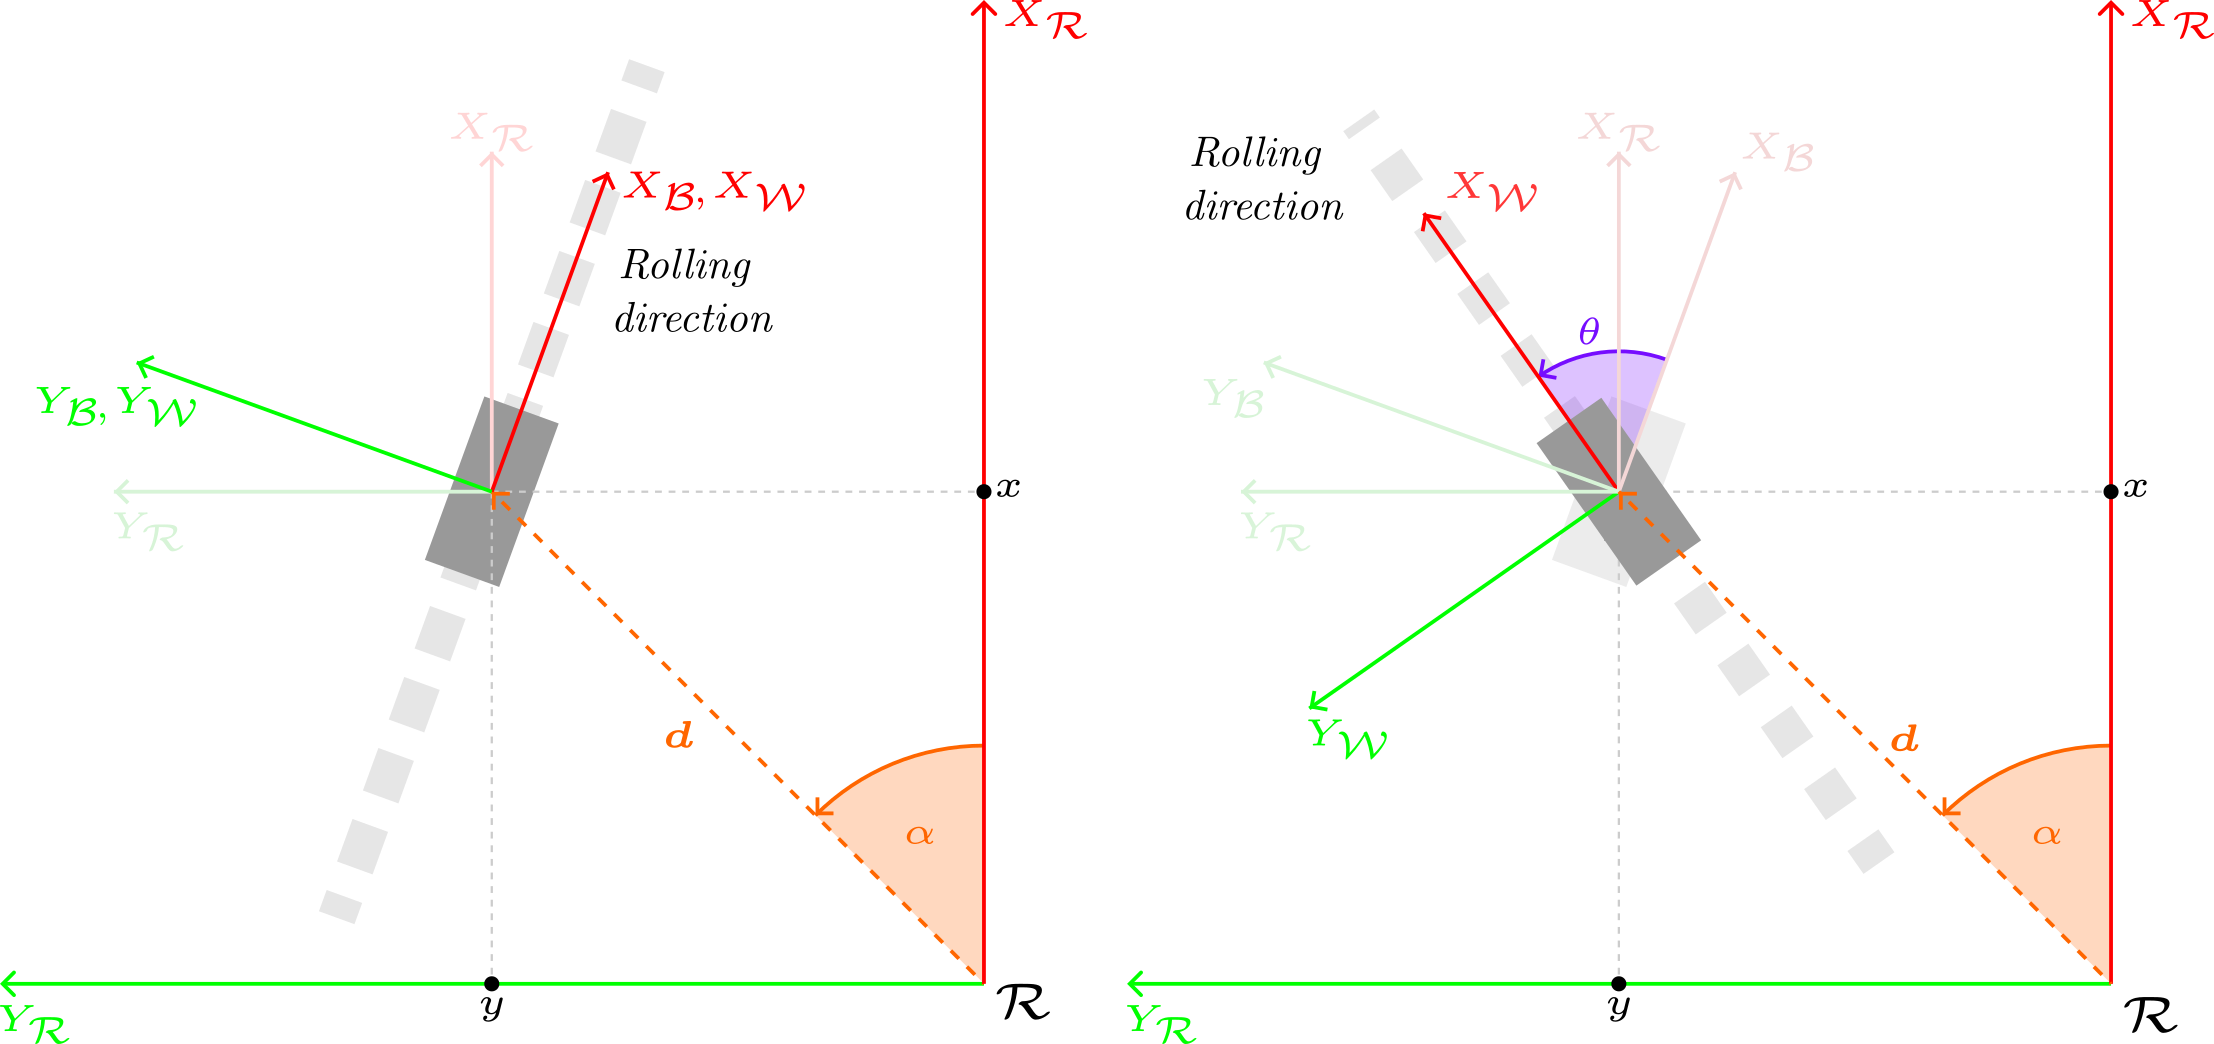
\includegraphics[width=1.0\linewidth]{images/rolling_direction.png}
    \caption{Left: Non-steerable conventional wheel, with fixed rolling direction. Right: Steerable conventional wheel, with variable rolling direction, achieved by pivoting the wheel by an angle \(\theta\) relative to the wheel's base CS, \(\frameB\).}
    \label{fig:rolling-direction}
\end{figure}

The linear velocity of the base, expressed in the robot's CS, is denoted as:

\begin{equation}
    {}^\frameR \vect{V}_r = \begin{bmatrix} {}^\frameR V_{r,x} \\ {}^\frameR V_{r,y} \\ 0 \end{bmatrix}
    \label{eq:rigid-velocity}
\end{equation}

and is expressed in \si{\meter\per\second}. The angular velocity of the base is denoted as:

\begin{equation}
    \boldsymbol{\omega}_r = \begin{bmatrix} 0 \\ 0 \\ \omega_{r,z} \end{bmatrix}
    \label{eq:rigid-angular-velocity}
\end{equation}

and is expressed in \si{\radian\per\second}.

\begin{figure}[H]
    \centering
    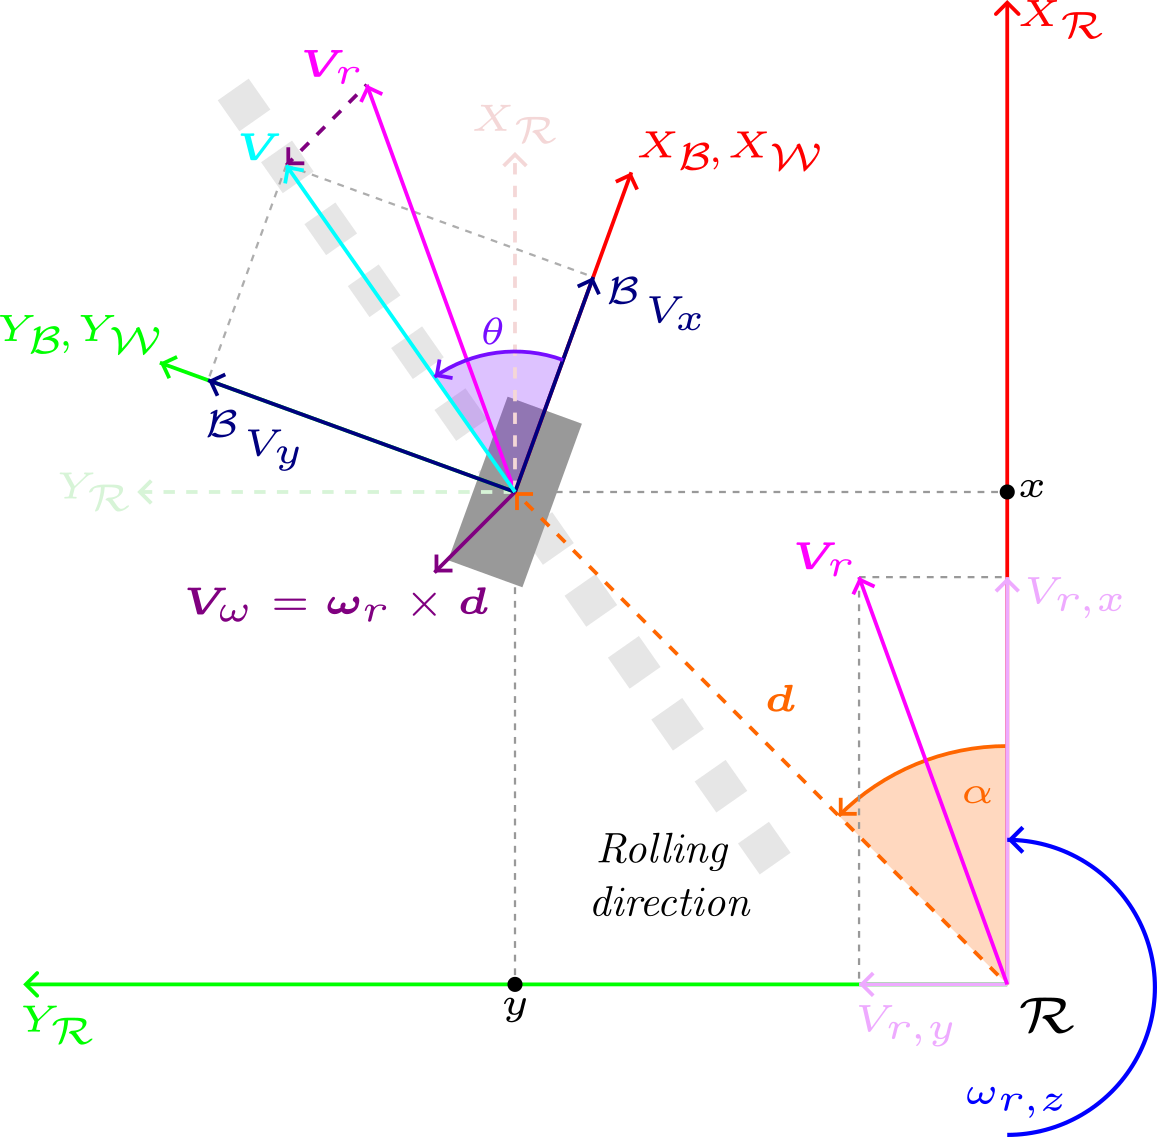
\includegraphics[width=1.0\linewidth]{images/wheel_vels.png}
    \caption{\(\vect{V}_r\) is the robot's velocity vector. \(\vect{V}_\omega\) is the tangential velocity vector of the wheel due to chassis rotation. \(\vect{V}\) is the velocity vector of the steerable wheel.}
    \label{fig:wheel-vels}
\end{figure}

The linear velocity of each wheel \(i\), expressed in the CS \(\frameR\), is denoted as:

\begin{equation}
    {}^\frameR \vect{V}_{i}  = {}^\frameR \vect{V}_r + \vect{\omega}_r \times {}^\frameR \vect{d}_{i} = {}^\frameR \vect{V}_r + \skewsym{\boldsymbol{\omega}_r}\,{}^\frameR \vect{d}_{i}
    \label{eq:wheel-velocity}
\end{equation}

where \({}^\frameR \vect{d}_{i}\) is the position vector of wheel \(i\) relative to the CS \(\frameR\), and \(\skewsym{\boldsymbol{\omega}_r}\) is the skew-symmetric operator representing the cross product with \(\boldsymbol{\omega}_r\). The cross product between \(\boldsymbol{\omega}_r\) and \({}^\frameR \vect{d}_{i}\) can be written as a matrix product using the skew-symmetric operator \([\cdot]_{\times}\): \(\boldsymbol{\omega}_r \times {}^\frameR \vect{d}_{i} = \skewsym{\boldsymbol{\omega}_r}\,{}^\frameR \vect{d}_{i}\), and \(\skewsym{\boldsymbol{\omega}_r}\) is defined as:

\begin{figure}[H]
    \centering
    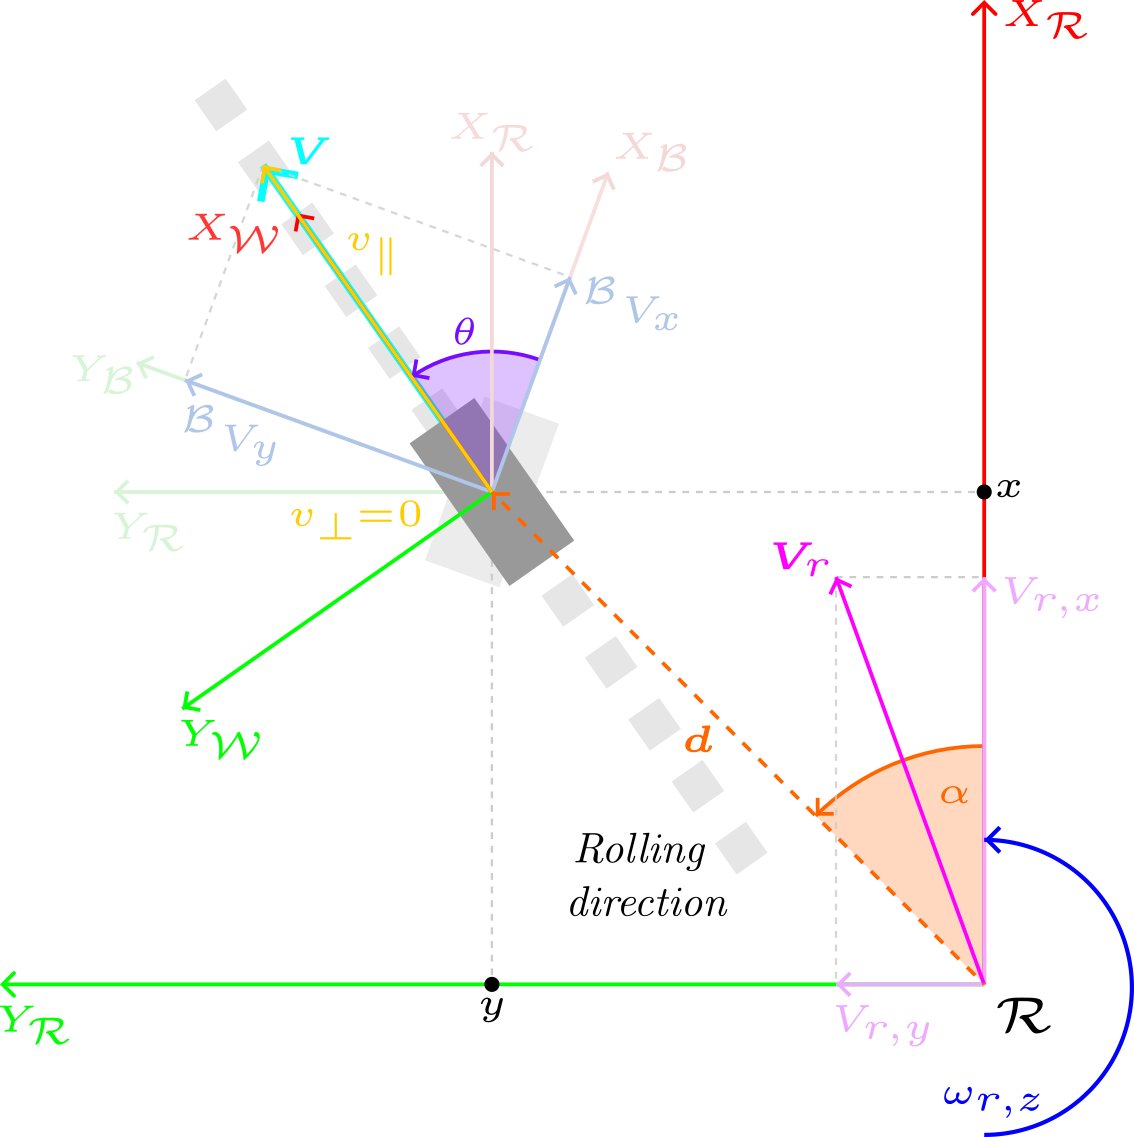
\includegraphics[width=1.0\linewidth]{images/wheel_vels_2.png}
    \caption{Relationship between the components of the wheel's velocity vector \(\vect{V}\) in the CS \(\frameB\), \({}^{\frameB}V_{x}\) and \({}^{\frameB}V_{y}\), and in the CS \(\frameW\), \(v_{\parallel}\) and \(v_{\perp}\).}
    \label{fig:wheel-vels-2}
\end{figure}

\begin{equation}
    \skewsym{\boldsymbol{\omega}_r} \triangleq
    \SkewFrom{\omega_{r,x}}{\omega_{r,y}}{\omega_{r,z}}
\end{equation}

\begin{equation}
    \begin{aligned}
        \boldsymbol{\omega}_r \times {}^\frameR \vect{d}_{i} & = \skewsym{\boldsymbol{\omega}_r}\,{}^\frameR \vect{d}_{i} \\
                                                             & = \begin{bmatrix}
                                                                     0            & -\omega_{r,z} & 0 \\
                                                                     \omega_{r,z} & \phantom{-}0  & 0 \\
                                                                     0            & \phantom{-}0  & 0
                                                                 \end{bmatrix} \begin{bmatrix}
                                                                                   d_{i}\cos\alpha_i \\
                                                                                   d_{i}\sin\alpha_i \\
                                                                                   0
                                                                               \end{bmatrix}                         \\
                                                             & = \begin{bmatrix}
                                                                     -\omega_{r,z} d_{i} \sin\alpha_i           \\
                                                                     \phantom{-}\omega_{r,z} d_{i} \cos\alpha_i \\
                                                                     0
                                                                 \end{bmatrix}
    \end{aligned}
\end{equation}

\begin{equation}
    \begin{aligned}
        {}^\frameR \vect{V}_{i}
        = {}^\frameR \vect{V}_r + \boldsymbol{\omega}_r \times {}^\frameR \vect{d}_i & = \begin{bmatrix}
                                                                                         {}^\frameR V_{r,x} - \omega_{r,z} d_{i} \sin\alpha_i \\
                                                                                         {}^\frameR V_{r,y} + \omega_{r,z} d_{i} \cos\alpha_i
                                                                                     \end{bmatrix} \\
                                                                                     & = \begin{bmatrix}
                                                                                             1 & 0 & -d_{i} \sin\alpha_i           \\
                                                                                             0 & 1 & \phantom{-}d_{i} \cos\alpha_i
                                                                                         \end{bmatrix} \begin{bmatrix}
                                                                                                           {}^\frameR V_{r,x} \\
                                                                                                           {}^\frameR V_{r,y} \\
                                                                                                           \omega_{r,z}
                                                                                                       \end{bmatrix}
    \end{aligned}
    \label{eq:wheel-velocity-expanded}
\end{equation}

The vector \({}^\frameR \vect{V}_{i}\) represents the linear velocity of wheel \(i\) expressed in the CS \(\frameR\). To apply the motion constraints to each wheel, its velocity must be expressed in its base CS, \(\frameBi\), \({}^{\frameBi} \vect{V}_{i}\).

\begin{equation}
    {}^{\frameBi} \vect{V}_{i} = {}^{\frameBi} R(\psi_i)_{\frameR} {}^\frameR \vect{V}_{i}
    \label{eq:vwheel-transform}
\end{equation}

where the rotation matrix \({}^{\frameBi} R(\psi_i)_{\frameR}\) represents the orientation of the CS \(\frameR\) in the CS \(\frameBi\), and is used to convert vectors expressed in the CS \(\frameR\) to the base CS of wheel \(i\), \(\frameBi\). The matrix known a priori is:

\begin{equation}
    {}^\frameR  R(\psi_i)_{\frameBi} =
    \begin{bmatrix}
        \cos\psi_i & -\sin\psi_i           \\
        \sin\psi_i & \phantom{-}\cos\psi_i
    \end{bmatrix}
\end{equation}

with \(\psi_i = \phi_i - \frac{\pi}{2} = \alpha_i + \beta_i - \frac{\pi}{2}\), representing the orientation of the CS \(\frameBi\) relative to the CS \(\frameR\). Since rotation matrices are orthonormal, their inverse is equal to their transpose, thus:

\begin{equation}
    {}^{\frameBi} R(\psi_i)_{\frameR} = \left({}^\frameR  R(\psi_i)_{\frameBi}\right)^{-1} = \left({}^\frameR  R(\psi_i)_{\frameBi}\right)^{\trans} =
    \begin{bmatrix}
        \phantom{-}\cos\psi_i & \sin\psi_i \\
        -\sin\psi_i           & \cos\psi_i
    \end{bmatrix}
\end{equation}

Next, the following trigonometric identities are applied to the matrix \({}^{\frameBi} R(\psi_i)_{\frameR}\):

\[
    \begin{aligned}
        \cos\psi_i & = \cos\left(\phi_i - \frac{\pi}{2}\right) = \phantom{-}\sin\phi_i \\
        \sin\psi_i & = \sin\left(\phi_i - \frac{\pi}{2}\right) = -\cos\phi_i
    \end{aligned}
\]

finally yielding:

\begin{equation}
    {}^{\frameBi}  R(\phi_i)_{\frameR} =
    \begin{bmatrix}
        \sin\phi_i & -\cos\phi_i           \\
        \cos\phi_i & \phantom{-}\sin\phi_i
    \end{bmatrix}
\end{equation}

\begin{equation}
    \begin{aligned}
        {}^{\frameBi} \vect{V}_i = \begin{bmatrix}
                                       {}^{\frameBi}V_{i,x} \\
                                       {}^{\frameBi}V_{i,y}
                                   \end{bmatrix} & = {}^{\frameBi}  R(\phi_i)_{\frameR} {}^\frameR \vect{V}_{i} \\
                                                   & = \begin{bmatrix}
                                                           \sin\phi_i & -\cos\phi_i           \\
                                                           \cos\phi_i & \phantom{-}\sin\phi_i
                                                       \end{bmatrix} \begin{bmatrix}
                                                                         1 & 0 & -d_{i} \sin\alpha_i           \\
                                                                         0 & 1 & \phantom{-}d_{i} \cos\alpha_i
                                                                     \end{bmatrix} \begin{bmatrix}
                                                                                       {}^\frameR V_{r,x} \\
                                                                                       {}^\frameR V_{r,y} \\
                                                                                       \omega_{r,z}
                                                                                   \end{bmatrix}
    \end{aligned}
\end{equation}

\begin{equation}
    \begin{bmatrix}
        {}^{\frameBi}V_{i,x} \\
        {}^{\frameBi}V_{i,y}
    \end{bmatrix} = \begin{bmatrix}
        \sin\phi_i & -\cos\phi_i           \\
        \cos\phi_i & \phantom{-}\sin\phi_i
    \end{bmatrix} \begin{bmatrix}
        1 & 0 & -d_{i} \sin\alpha_i           \\
        0 & 1 & \phantom{-}d_{i} \cos\alpha_i
    \end{bmatrix} \begin{bmatrix}
        {}^\frameR V_{r,x} \\
        {}^\frameR V_{r,y} \\
        \omega_{r,z}
    \end{bmatrix}
    \label{eq:wheel-constraints-compact}
\end{equation}

\[
    \begin{bmatrix}
        {}^{\frameBi}V_{i,x} \\
        {}^{\frameBi}V_{i,y}
    \end{bmatrix} = \begin{bmatrix}
        \sin\phi_i & -\cos\phi_i           & -d_i(\phantom{-}\sin\alpha_i\sin\phi_i + \cos\alpha_i\cos\phi_i) \\
        \cos\phi_i & \phantom{-}\sin\phi_i & \phantom{-}d_i(-\sin\alpha_i\cos\phi_i + \cos\alpha_i\sin\phi_i)
    \end{bmatrix} \begin{bmatrix}
        {}^{\frameR}V_{r,x} \\
        {}^{\frameR}V_{r,y} \\
        \omega_{r,z}
    \end{bmatrix}
\]

Next, the following trigonometric identities are applied:

\[
    \begin{aligned}
        \phantom{-}\sin\alpha_i\sin\phi_i + \cos\alpha_i\cos\phi_i & = \cos(\phi_i - \alpha_i) = \cos((\alpha_i + \beta_i) - \alpha_i) = \cos\beta_i \\
        -\sin\alpha_i\cos\phi_i + \cos\alpha_i\sin\phi_i           & = \sin(\phi_i - \alpha_i) = \sin((\alpha_i + \beta_i) - \alpha_i) = \sin\beta_i
    \end{aligned}
\]

Finally resulting in:

\begin{equation}
    \begin{bmatrix}
        {}^{\frameBi}V_{i,x} \\
        {}^{\frameBi}V_{i,y}
    \end{bmatrix} = \begin{bmatrix}
        \sin\phi_i & -\cos\phi_i           & -d_i\cos\beta_i           \\
        \cos\phi_i & \phantom{-}\sin\phi_i & \phantom{-}d_i\sin\beta_i
    \end{bmatrix} \begin{bmatrix}
        {}^\frameR V_{r,x} \\
        {}^\frameR V_{r,y} \\
        \omega_{r,z}
    \end{bmatrix}
    \label{eq:wheel-constraints-final}
\end{equation}

For each wheel \(i\), a system of 2 linear equations with 3 unknowns (\({}^\frameR V_{r,x}\), \({}^\frameR V_{r,y}\), and \(\omega_{r,z}\)) is obtained. In general, for \(N\) wheels, \(2N\) linear equations and 3 unknowns are obtained. Therefore, for \(N \ge 2\), the system is overdetermined. Equation \ref{eq:wheel-constraints-final} provides the wheel velocity expressed in its base CS \(\frameBi\). However, the physical motion constraints of the wheel originated by its contact with the ground apply in the wheel's own CS, \(\frameWi\). For this reason, it is necessary to define the intrinsic velocity components of the wheel:

\begin{itemize}
    \item \(v_{i\parallel}\): the velocity component aligned with the rolling direction (axis \(\ejeXWi\)).
    \item \(v_{i\perp}\): the velocity component perpendicular to the rolling direction (axis \(\ejeYWi\); \textit{i.e.}, the direction of its rotation axis).
\end{itemize}

Depending on whether the wheels used on a platform are non-steerable conventional, steerable conventional, mecanum, or omnidirectional, the geometric relationship between the components of the wheel's velocity vector \(\vect{V}\) in the base CS (\({}^{\frameBi}V_{i,x}, {}^{\frameBi}V_{i,y}\)) and in the wheel-fixed CS (\(v_{i\parallel}, v_{i\perp}\)) will change. See Figure \ref{fig:wheel-vels-2}. Depending on the platform, different physical constraints will apply to the components \(v_{i\parallel}\) and \(v_{i\perp}\), yielding specific expressions that solve the forward and inverse kinematics for the considered platform.

\section{General considerations on forward and inverse kinematics}
\label{sec:general-considerations}

In general, the forward and inverse kinematics of a terrestrial robot is defined by a matrix expression of the form:

\begin{equation}
    A\mathbf{x}=\mathbf{b}
\end{equation}

where:

\[
    A \in \mathbb{R}^{2N \times 3}, \quad \mathbf{x} \in \mathbb{R}^3, \quad \mathbf{b} \in \mathbb{R}^{2N}
\]

\[
    A = \begin{bmatrix}
        \sin\phi_0     & -\cos\phi_0               & -d_0\cos\beta_0                   \\
        \cos\phi_0     & \phantom{-}\sin\phi_0     & \phantom{-}d_0\sin\beta_0         \\
        \vdots         & \vdots                    & \vdots                            \\
        \sin\phi_{N-1} & -\cos\phi_{N-1}           & -d_{N-1}\cos\beta_{N-1}           \\
        \cos\phi_{N-1} & \phantom{-}\sin\phi_{N-1} & \phantom{-}d_{N-1}\sin\beta_{N-1}
    \end{bmatrix}, \quad \mathbf{x} =
    \begin{bmatrix}
        {}^\frameR V_{r,x} \\
        {}^\frameR V_{r,y} \\
        \omega_{r,z}
    \end{bmatrix}, \quad \mathbf{b} = \begin{bmatrix}
        {}^{\frameBZero}V_{0,x}        \\
        {}^{\frameBZero}V_{0,y}        \\
        \vdots                         \\
        {}^{\frameBNMinusOne}V_{N-1,x} \\
        {}^{\frameBNMinusOne}V_{N-1,y}
    \end{bmatrix}
\]

Given that for any robot with \(N \ge 2\) wheels, \(2N\) equations and only 3 unknowns are obtained, we are dealing with an overdetermined linear system. In a purely mathematical ideal scenario, it would suffice to take any subset of 3 linearly independent equations to solve the system and find the chassis velocity, \(\mathbf{x}\). However, in the real implementation of a terrestrial robot, the equations never match perfectly due to imperfections such as:

\begin{itemize}
    \item Noise and quantization in sensor (encoder) readings.
    \item Small wheel slips on the ground.
    \item Slight deviations in the geometric calibration of the base.
\end{itemize}

Therefore, the system is not solved by seeking an exact algebraic solution, but rather by finding the estimate \(\hat{\mathbf{x}}\) that minimizes the global squared error of all wheels simultaneously:

\begin{equation}
    \hat{\mathbf{x}} = \arg\min_{\mathbf{x}} \|A\mathbf{x} - \mathbf{b}\|^2
\end{equation}

The solution to this least squares problem is given by the expression known as Normal Equations, which is obtained from a process of searching for the minimum of the error function (differentiating and setting to zero):

\begin{equation}
    A^{\trans} A \mathbf{x} = A^{\trans} \mathbf{b}
\end{equation}

Therefore, the optimal solution is obtained through:

\begin{equation}
    \hat{\mathbf{x}} = (A^{\trans}A)^{-1}A^{\trans}\mathbf{b} = A^+\mathbf{b}
\end{equation}

where \(A^+\) is called the Moore-Penrose pseudoinverse of matrix \(A\).

From a computational numerical calculation standpoint, directly inverting the matrix \((A^{\trans}A)\) can be unstable if the original matrix \(A\) is ill-conditioned. A matrix is considered ill-conditioned when small variations or noise in the input data (the vector \(\mathbf{b}\)) are drastically amplified, causing erratic calculations in the resulting solution \(\hat{\mathbf{x}}\). The numerical misbehavior that can arise when using the normal equations formula is due to the fact that the term \((A^{\trans}A)^{-1}\allowbreak A^{\trans}\) squares the singular values of \(A\). If \(A\) has a small singular value, close to zero, squaring it makes it even smaller. When attempting to invert that value, the computer divides by a near-zero number, causing the results to spiral to infinity and all precision in the solution to be lost.

Although not strictly necessary for kinematics development, for completeness it is noted that to ascertain the geometric robustness of matrix \(A\), the ratio between its maximum and minimum singular values (\(\kappa = \frac{\sigma_{\max}}{\sigma_{\min}}\)) is used, known as the \textbf{condition number}, \(\kappa(A)\). As a reference:

\begin{itemize}
    \item \(\kappa = 1\): \(A\) is the perfect matrix (example: the Identity matrix or a pure rotation matrix). There is no loss of precision.
    \item \(1 < \kappa < 10^2\): \(A\) is well-conditioned. The system is robust; sensor errors will not be significantly amplified.
    \item \(10^3 < \kappa < 10^6\): \(A\) is moderately ill-conditioned. Caution must be exercised, as simple methods like inverting \((A^{\trans}A)\) may start to yield imprecise results.
    \item \(\kappa \approx 10^{12} \text{ to } 10^{15}\): \(A\) is ill-conditioned. The matrix is nearly singular (its rows/columns are almost dependent).
    \item \(\kappa > 10^{16}\): \(A\) is singular and unusable. For a computer working with double precision (64 bits), this means the matrix cannot be reliably inverted.
\end{itemize}

To avoid these numerical stability issues that could arise, in practice, the pseudoinverse \(A^+\) is obtained by applying Singular Value Decomposition (SVD) to the original matrix \(A\). SVD is the most robust and secure numerical method, as it entirely avoids the product \((A^{\trans}A)\) and is capable of handling near-singular matrices (situations where the robot's geometric equations are so similar or redundant that the system is on the verge of not being invertible) without the resulting calculations spiraling to infinity. This method works even if matrix \(A\) does not have full rank (if some of the equations are directly contradictory).

However, it is fundamental to make a critical distinction between the software's mathematical robustness and the robot's physical viability. If, when evaluating the constant geometric matrix \(A\) during the design phase, a high condition number is obtained (for example, \(\kappa > 10^3\), and critically if \(\kappa > 10^6\)), \textbf{it will happen that, although the SVD algorithm prevents a program crash by returning a stable mathematical solution (by truncating near-null values), in reality, a severe flaw in the mechanical design is being masked.} Physically, this means that the constructive arrangement of the wheels (their distances \(d_i\) or mounting angles \(\alpha_i, \beta_i\)) generates a degenerate kinematics, where the chassis loses the ability to move independently in all its degrees of freedom, or where rolling directions directly conflict. In this scenario, even if the software delivers a seemingly valid numerical result, the physical robot will suffer uncontrollable drifts, mechanical stress, and erratic movements at the slightest noise in the encoders. Therefore, SVD should not be used as an excuse to ignore bad geometry; if the initial condition number is excessively high, the inevitable solution involves redesigning the wheel placement and base orientation in the CAD design until a well-conditioned system is achieved (ideally \(\kappa \le 100\)).

SVD decomposes the matrix into \(A = U \Sigma V^{\trans}\), allowing the pseudoinverse to be constructed directly as \(A^+ = V \Sigma^+ U^{\trans}\).

\textbf{Proof:}

If \(A = U \Sigma V^{\trans}\), the transpose property for a matrix product is applied: \((X Y Z)^{\trans} = Z^{\trans} Y^{\trans} X^{\trans}\) (the order is reversed).

\begin{equation}
    A^{\trans} = (V^{\trans})^{\trans} \Sigma^{\trans} U^{\trans}
\end{equation}

Transposing twice returns the original matrix (\((V^{\trans})^{\trans} = V\)), and since \(\Sigma\) is a diagonal matrix that does not change upon transposing (\(\Sigma^{\trans} = \Sigma\))\footnote{For the equality \(\Sigma^{\trans} = \Sigma\) to be strictly true, \(\Sigma\) must be a square matrix. In overdetermined systems, where \(A\) is a rectangular \(M \times N\) matrix, the original \(\Sigma\) matrix is rectangular \(M \times N\) and \(\Sigma^{\trans}\) would be \(N \times M\), hence the equality would not hold. However, in practice, the Reduced SVD (or \textit{Thin SVD}) is typically employed to solve these systems, which trims the rows of zeros from the \(\Sigma\) matrix, converting it into a square \(N \times N\) matrix. In this way, \(\Sigma^{\trans} = \Sigma\) does hold in the Reduced SVD, allowing the formula \(A^+ = V \Sigma^+ U^{\trans}\) to be developed without dimensional conflicts. In the Eigen library for C++, combining the options \texttt{ComputeThinU | ComputeThinV} performs precisely this calculation.}, we obtain:

\begin{equation}
    A^{\trans} = V \Sigma U^{\trans}
\end{equation}

Substituting into the product \(A^{\trans} A\):

\begin{equation}
    A^{\trans} A = (V \Sigma U^{\trans}) (U \Sigma V^{\trans})
\end{equation}

By the associative property of matrices, the inner parentheses can be omitted:

\begin{equation}
    A^{\trans} A = V \Sigma (U^{\trans} U) \Sigma V^{\trans}
\end{equation}

Matrix \(U\) is orthogonal, meaning its transpose multiplied by itself results in the Identity matrix (\(U^{\trans} U = I\)):

\begin{equation}
    A^{\trans} A = V \Sigma I \Sigma V^{\trans}
\end{equation}

Multiplying by the Identity matrix does not alter the result, and \(\Sigma\) multiplied by itself is \(\Sigma^2\) (which is equivalent to squaring the values of its diagonal):

\begin{equation}
    A^{\trans} A = V \Sigma^2 V^{\trans}
\end{equation}

Next, the inverse is applied to the entire expression using the inverse property for a product: \((X Y Z)^{-1} = Z^{-1} Y^{-1} X^{-1}\).

\begin{equation}
    (A^{\trans} A)^{-1} = (V^{\trans})^{-1} (\Sigma^2)^{-1} V^{-1}
\end{equation}

Since \(V\) is also an orthogonal matrix, its inverse is equal to its transpose, \(V^{-1} = V^{\trans}\), and thus, \((V^{\trans})^{-1} = V\). The inverse of a diagonal matrix \(\Sigma^2\) is simply denoted as \(\Sigma^{-2}\) (which consists of inverting the squared values of its diagonal). Substituting these properties yields:

\begin{equation}
    (A^{\trans} A)^{-1} = V \Sigma^{-2} V^{\trans}
\end{equation}

It is now multiplied by \(A^{\trans}\) from the right to complete the Normal Equations expression:

\begin{equation}
    (A^{\trans} A)^{-1} A^{\trans} = (V \Sigma^{-2} V^{\trans}) (V \Sigma U^{\trans})
\end{equation}

The inner parentheses are removed again via the associative property:

\begin{equation}
    (A^{\trans} A)^{-1} A^{\trans} = V \Sigma^{-2} (V^{\trans} V) \Sigma U^{\trans}
\end{equation}

Once more, given that \(V\) is orthogonal, \(V^{\trans} V = I\). The central term disappears:

\begin{equation}
    (A^{\trans} A)^{-1} A^{\trans} = V \Sigma^{-2} \Sigma U^{\trans}
\end{equation}

At this point, we have \(\Sigma^{-2}\) multiplied by \(\Sigma\). Because both are diagonal matrices, the operation is equivalent to multiplying each element of the \(\Sigma^{-2}\) diagonal by the corresponding element of the \(\Sigma\) diagonal. So each element of the resulting diagonal is the original \(\Sigma\) value raised to \(-2 + 1 = -1\) (that is, the reciprocal of the original \(\Sigma\) values). This resulting diagonal matrix is denoted as \(\Sigma^+\):

\begin{itemize}
    \item If \(A\) does \textbf{not} have full rank, \(\Sigma^+\) is defined as the diagonal matrix containing the reciprocals of the non-zero singular values of \(A\), and zeros in the positions corresponding to the zero singular values.
    \item If \(A\) \textbf{has} full rank, then \(\Sigma^+\) is actually \(\Sigma^{-1}\) (a proper inverse), which is the diagonal matrix containing the reciprocals of all the singular values of \(A\).
\end{itemize}

Finally, substituting \(\Sigma^+\), the expression is reached:

\begin{equation}
    (A^{\trans} A)^{-1} A^{\trans} = V \Sigma^+ U^{\trans}
\end{equation}

As previously discussed, the computational problem arises when the computer directly evaluates the expression \((A^{\trans} A)^{-1}\), since it must square singular values that could be very close to zero. When attempting to invert those nearly zero squared values, numerical overflows occur. By using the direct final formula \(V \Sigma^+ U^{\trans}\) provided by SVD, the algorithm only inverts the original values (\(\Sigma^+\)), keeping the system stable at all times.

\section{Kinematics of a three swerve drive robot}

The base with three steerable active wheels (three swerve drive) is an omnidirectional locomotion system. It allows a terrestrial robot to move in any direction without first having to change the chassis orientation. Each wheel is steered independently, so the robot gains maneuverability and flexibility.

\begin{figure}[H]
    \centering
    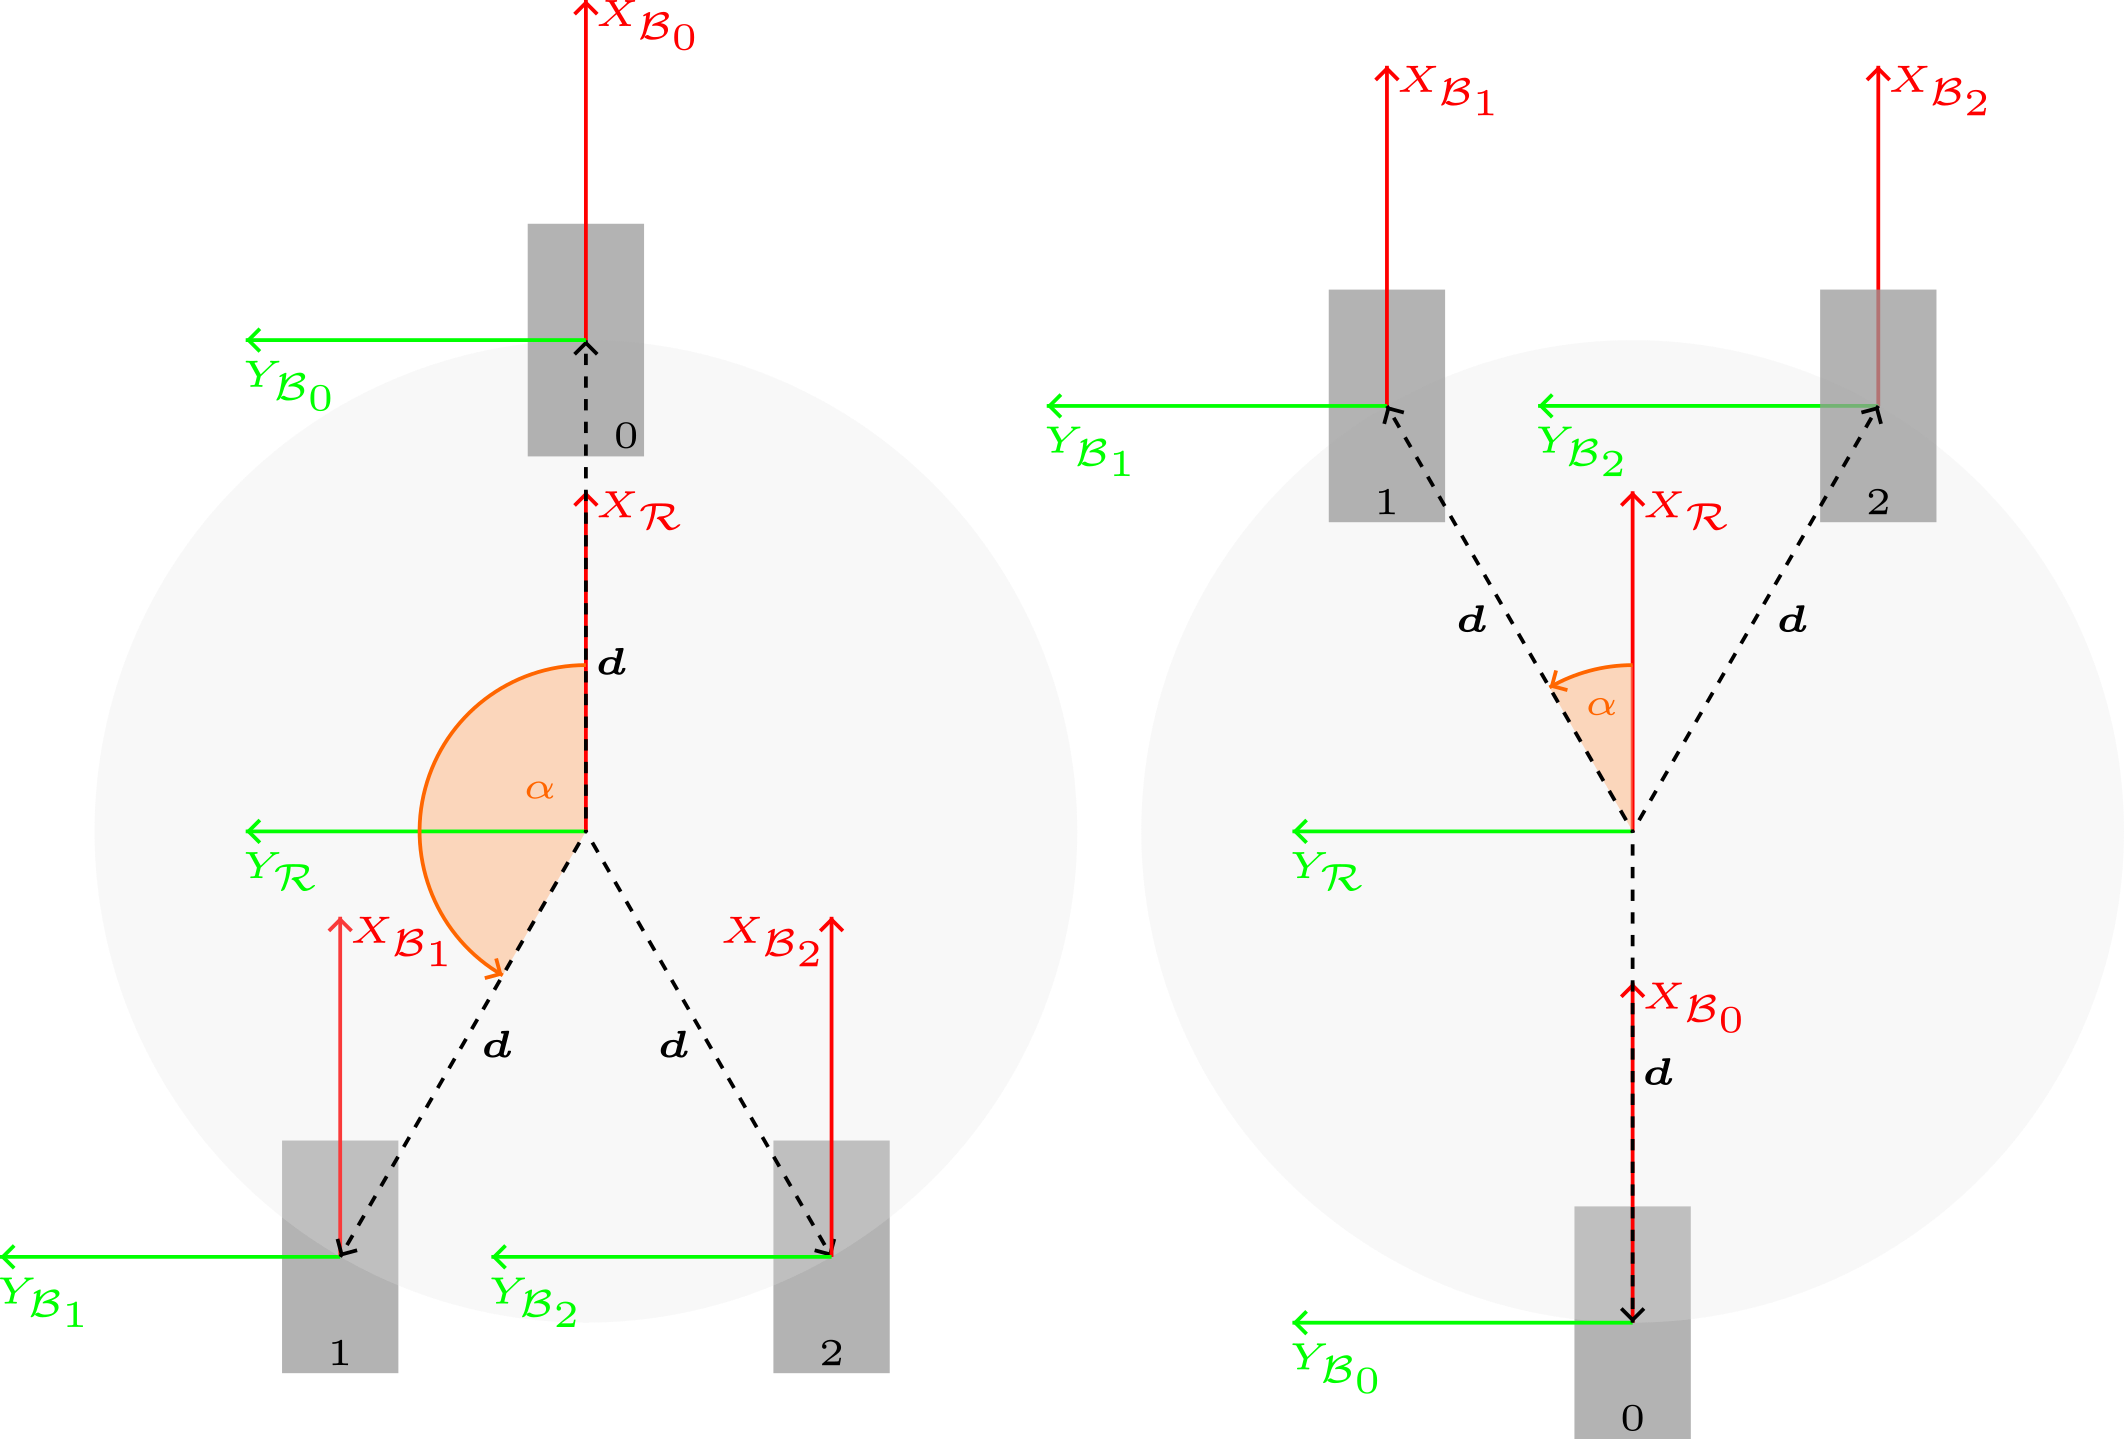
\includegraphics[width=1.0\linewidth]{images/three_swerve_drive_configuration.png}
    \caption{Common wheel configurations in a three swerve drive system (left: inverted-Y configuration, right: Y configuration)}
    \label{fig2:three-swerve-drive-configuration}
\end{figure}

All wheels have the same radius \(r\) and are located at the same distance \(d\) from the center of the base. Furthermore, in this particular case, it is imposed:

\[
    \begin{aligned}
        \psi_i = \phi_i - \frac{\pi}{2} = 0 \quad          & \Longrightarrow \quad \phi_i = \frac{\pi}{2}             \\
        \phi_i = \alpha_i + \beta_i = \frac{\pi}{2}, \quad & \Longrightarrow \quad \beta_i = \frac{\pi}{2} - \alpha_i
    \end{aligned}
\]

and therefore:

\[
    {}^{\frameBi} R\left(\phi_i = \frac{\pi}{2}\right)_{\frameR} = \begin{bmatrix}
        \sin\frac{\pi}{2} & -\cos\frac{\pi}{2}           \\
        \cos\frac{\pi}{2} & \phantom{-}\sin\frac{\pi}{2}
    \end{bmatrix} = \begin{bmatrix}
        1 & 0 \\
        0 & 1
    \end{bmatrix}
\]

For the inverted-Y configuration:

\begin{itemize}
    \item \(\alpha \in \left[\frac{\pi}{2}, \pi\right)\) and \(d > 0\)
    \item Front wheel \((i = 0)\):
          \[
              \begin{aligned}
                  \alpha_0   & = 0                                                              \\
                  \vect{d}_0 & = (d\cos\alpha_0,\ d\sin\alpha_0) = (d\cos 0,\ d\sin 0) = (d, 0) \\
                  \beta_0    & = \frac{\pi}{2} - \alpha_0 = \frac{\pi}{2} - 0 = \frac{\pi}{2}
              \end{aligned}
          \]
    \item Left wheel \((i = 1)\):
          \[
              \begin{aligned}
                  \alpha_1   & = \alpha                                                      \\
                  \vect{d}_1 & = (d\cos\alpha_1, d\sin\alpha_1) = (d\cos\alpha, d\sin\alpha) \\
                  \beta_1    & = \frac{\pi}{2} - \alpha_1 = \frac{\pi}{2} - \alpha
              \end{aligned}
          \]
    \item Right wheel \((i = 2)\):
          \[
              \begin{aligned}
                  \alpha_2   & = -\alpha                                                                                         \\
                  \vect{d}_2 & = (d\cos\alpha_2, d\sin\alpha_2) = (d\cos(-\alpha), d\sin(-\alpha)) = (d\cos\alpha, -d\sin\alpha) \\
                  \beta_2    & = \frac{\pi}{2} - \alpha_2 = \frac{\pi}{2} - (-\alpha) = \frac{\pi}{2} + \alpha
              \end{aligned}
          \]
\end{itemize}

The matrix \(A\) for the inverted-Y configuration is presented below:

\begin{equation}
    \begin{aligned}
        A & = \begin{bmatrix}
                  \sin\phi_0 & -\cos\phi_0           & -d_0\cos\beta_0           \\
                  \cos\phi_0 & \phantom{-}\sin\phi_0 & \phantom{-}d_0\sin\beta_0 \\
                  \sin\phi_1 & -\cos\phi_1           & -d_1\cos\beta_1           \\
                  \cos\phi_1 & \phantom{-}\sin\phi_1 & \phantom{-}d_1\sin\beta_1 \\
                  \sin\phi_2 & -\cos\phi_2           & -d_2\cos\beta_2           \\
                  \cos\phi_2 & \phantom{-}\sin\phi_2 & \phantom{-}d_2\sin\beta_2
              \end{bmatrix} = \begin{bmatrix}
                                  1 & 0 & -d\cos\left(\frac{\pi}{2}- \alpha_0\right)            \\
                                  0 & 1 & \phantom{-}d\sin\left(\frac{\pi}{2} - \alpha_0\right) \\
                                  1 & 0 & -d\cos\left(\frac{\pi}{2}-\alpha_1\right)             \\
                                  0 & 1 & \phantom{-}d\sin\left(\frac{\pi}{2}-\alpha_1\right)   \\
                                  1 & 0 & -d\cos\left(\frac{\pi}{2}-\alpha_2\right)             \\
                                  0 & 1 & \phantom{-}d\sin\left(\frac{\pi}{2}-\alpha_2\right)
                              \end{bmatrix}  = \\
          & = \begin{bmatrix}
                  1 & 0 & -d\sin\alpha_0           \\
                  0 & 1 & \phantom{-}d\cos\alpha_0 \\
                  1 & 0 & -d\sin\alpha_1           \\
                  0 & 1 & \phantom{-}d\cos\alpha_1 \\
                  1 & 0 & -d\sin\alpha_2           \\
                  0 & 1 & \phantom{-}d\cos\alpha_2
              \end{bmatrix} = \begin{bmatrix}
                                  1 & 0 & -y_0           \\
                                  0 & 1 & \phantom{-}x_0 \\
                                  1 & 0 & -y_1           \\
                                  0 & 1 & \phantom{-}x_1 \\
                                  1 & 0 & -y_2           \\
                                  0 & 1 & \phantom{-}x_2
                              \end{bmatrix}
    \end{aligned}
\end{equation}

For the Y configuration:

\begin{itemize}
    \item \(\alpha \in \left(0, \frac{\pi}{2}\right]\) and \(d > 0\)
    \item Rear wheel \((i = 0)\):
          \[
              \begin{aligned}
                  \alpha_0   & = \pi                                                             \\
                  \vect{d}_0 & = (d\cos\alpha_0, d\sin\alpha_0) = (d\cos\pi, d\sin\pi) = (-d, 0) \\
                  \beta_0    & = \frac{\pi}{2} - \alpha_0 = \frac{\pi}{2} - \pi = -\frac{\pi}{2}
              \end{aligned}
          \]
    \item Left wheel \((i = 1)\):
          \[
              \begin{aligned}
                  \alpha_1   & = \alpha                                                      \\
                  \vect{d}_1 & = (d\cos\alpha_1, d\sin\alpha_1) = (d\cos\alpha, d\sin\alpha) \\
                  \beta_1    & = \frac{\pi}{2} - \alpha_1 = \frac{\pi}{2} - \alpha
              \end{aligned}
          \]
    \item Right wheel \((i = 2)\):
          \[
              \begin{aligned}
                  \alpha_2   & = -\alpha                                                                                         \\
                  \vect{d}_2 & = (d\cos\alpha_2, d\sin\alpha_2) = (d\cos(-\alpha), d\sin(-\alpha)) = (d\cos\alpha, -d\sin\alpha) \\
                  \beta_2    & = \frac{\pi}{2} - \alpha_2 = \frac{\pi}{2} - (-\alpha) = \frac{\pi}{2} + \alpha
              \end{aligned}
          \]
\end{itemize}

The matrix \(A\) for the Y configuration is presented below:

\begin{equation}
    \begin{aligned}
        A & = \begin{bmatrix}
                  \sin\phi_0 & -\cos\phi_0           & -d_0\cos\beta_0           \\
                  \cos\phi_0 & \phantom{-}\sin\phi_0 & \phantom{-}d_0\sin\beta_0 \\
                  \sin\phi_1 & -\cos\phi_1           & -d_1\cos\beta_1           \\
                  \cos\phi_1 & \phantom{-}\sin\phi_1 & \phantom{-}d_1\sin\beta_1 \\
                  \sin\phi_2 & -\cos\phi_2           & -d_2\cos\beta_2           \\
                  \cos\phi_2 & \phantom{-}\sin\phi_2 & \phantom{-}d_2\sin\beta_2
              \end{bmatrix} = \begin{bmatrix}
                                  1 & 0 & -d\cos\left(\frac{\pi}{2} - \alpha_0\right)           \\
                                  0 & 1 & \phantom{-}d\sin\left(\frac{\pi}{2} - \alpha_0\right) \\
                                  1 & 0 & -d\cos\left(\frac{\pi}{2} - \alpha_1\right)           \\
                                  0 & 1 & \phantom{-}d\sin\left(\frac{\pi}{2} - \alpha_1\right) \\
                                  1 & 0 & -d\cos\left(\frac{\pi}{2} - \alpha_2\right)           \\
                                  0 & 1 & \phantom{-}d\sin\left(\frac{\pi}{2} - \alpha_2\right)
                              \end{bmatrix}  = \\
          & = \begin{bmatrix}
                  1 & 0 & -d\sin\alpha_0           \\
                  0 & 1 & \phantom{-}d\cos\alpha_0 \\
                  1 & 0 & -d\sin\alpha_1           \\
                  0 & 1 & \phantom{-}d\cos\alpha_1 \\
                  1 & 0 & -d\sin\alpha_2           \\
                  0 & 1 & \phantom{-}d\cos\alpha_2
              \end{bmatrix} = \begin{bmatrix}
                                  1 & 0 & -y_0           \\
                                  0 & 1 & \phantom{-}x_0 \\
                                  1 & 0 & -y_1           \\
                                  0 & 1 & \phantom{-}x_1 \\
                                  1 & 0 & -y_2           \\
                                  0 & 1 & \phantom{-}x_2
                              \end{bmatrix}
    \end{aligned}
\end{equation}

Therefore, it is demonstrated that both configurations, inverted-Y and Y, share the same matrix \(A\), which implies that their forward and inverse kinematics are identical. The only difference between both configurations lies in the physical arrangement of the wheels, but kinematically, both are equivalent.

\subsection{Inverse kinematics of the three swerve}

For a steerable conventional wheel, the following holds:

\begin{equation}
    {}^{\frameWi}\vect{V}_{i} = \begin{bmatrix}
        v_{i\parallel} \\
        v_{i\perp}
    \end{bmatrix} = \begin{bmatrix}
        \omega_i r \\
        0
    \end{bmatrix}
\end{equation}

where \(v_{i\parallel}\) is the velocity of wheel \(i\) in the rolling direction and \(v_{i\perp}\) is the component perpendicular to the rolling direction, which is zero, since the wheel cannot slip laterally. Given that the steerable wheel must rotate by an angle \(\theta_i\) relative to its base CS \(\frameBi\) to align its rolling direction (axis \(X_{\frameWi}\)) with the wheel velocity vector \(\vect{V}_i\), it is evident that:

\begin{equation}
    v_{i\parallel} = \|{}^{\frameBi} \vect{V}_i\| = \sqrt{{}^{\frameBi}V_{i,x}^2 + {}^{\frameBi}V_{i,y}^2} = r\omega_i
    \label{eq:tsd-v_parallel}
\end{equation}

\begin{figure}[H]
    \centering
    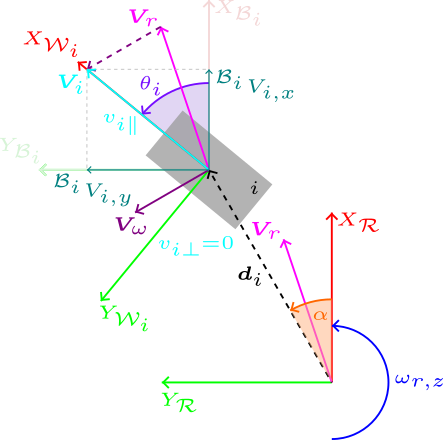
\includegraphics[width=0.8\linewidth]{images/three_swerve_drive_steerable_wheel.png}
    \caption{Steerable conventional wheel aligned with its velocity vector \(\vect{V}_i\) via a rotation of angle \(\theta_i\) relative to its base CS \(\frameBi\). The rolling direction is defined by the \(X_{\frameWi}\) axis of the CS fixed to wheel \(i\), \(\frameWi\).}
    \label{fig2:tsd-steerable-wheel}
\end{figure}

Steps to calculate the inverse kinematics of a robot with a three swerve drive base:

\begin{itemize}
    \item Given the chassis velocity vector \({}^\frameR \vect{V}_r\), the velocity of each wheel \(i\) in its base CS \(\frameBi\), \({}^{\frameBi}\vect{V}_i\), is obtained by applying the coordinate transformation of Equation \ref{eq:wheel-constraints-final}.
    \item The steering angle \(\theta_i\) that each wheel \(i\) must adopt to align its rolling direction with the velocity vector \({}^{\frameBi} \vect{V}_i\) is calculated using the \(\arctan2\) function.
          \begin{equation}
              \theta_i = \arctan2({}^{\frameBi}V_{i,y}, {}^{\frameBi}V_{i,x})
              \label{eq:tsd-inverse-kinematics-angle}
          \end{equation}
    \item The angular velocity of each wheel \(i\) is calculated from Expression \ref{eq:tsd-v_parallel}.
          \begin{equation}
              \omega_i = \frac{v_{i\parallel}}{r} = \frac{\|{}^{\frameBi} \vect{V}_i\|}{r} = \frac{\sqrt{{}^{\frameBi}V_{i,x}^2 + {}^{\frameBi}V_{i,y}^2}}{r}
              \label{eq:tsd-inverse-kinematics-angular-speed}
          \end{equation}
\end{itemize}

\begin{figure}[H]
    \centering
    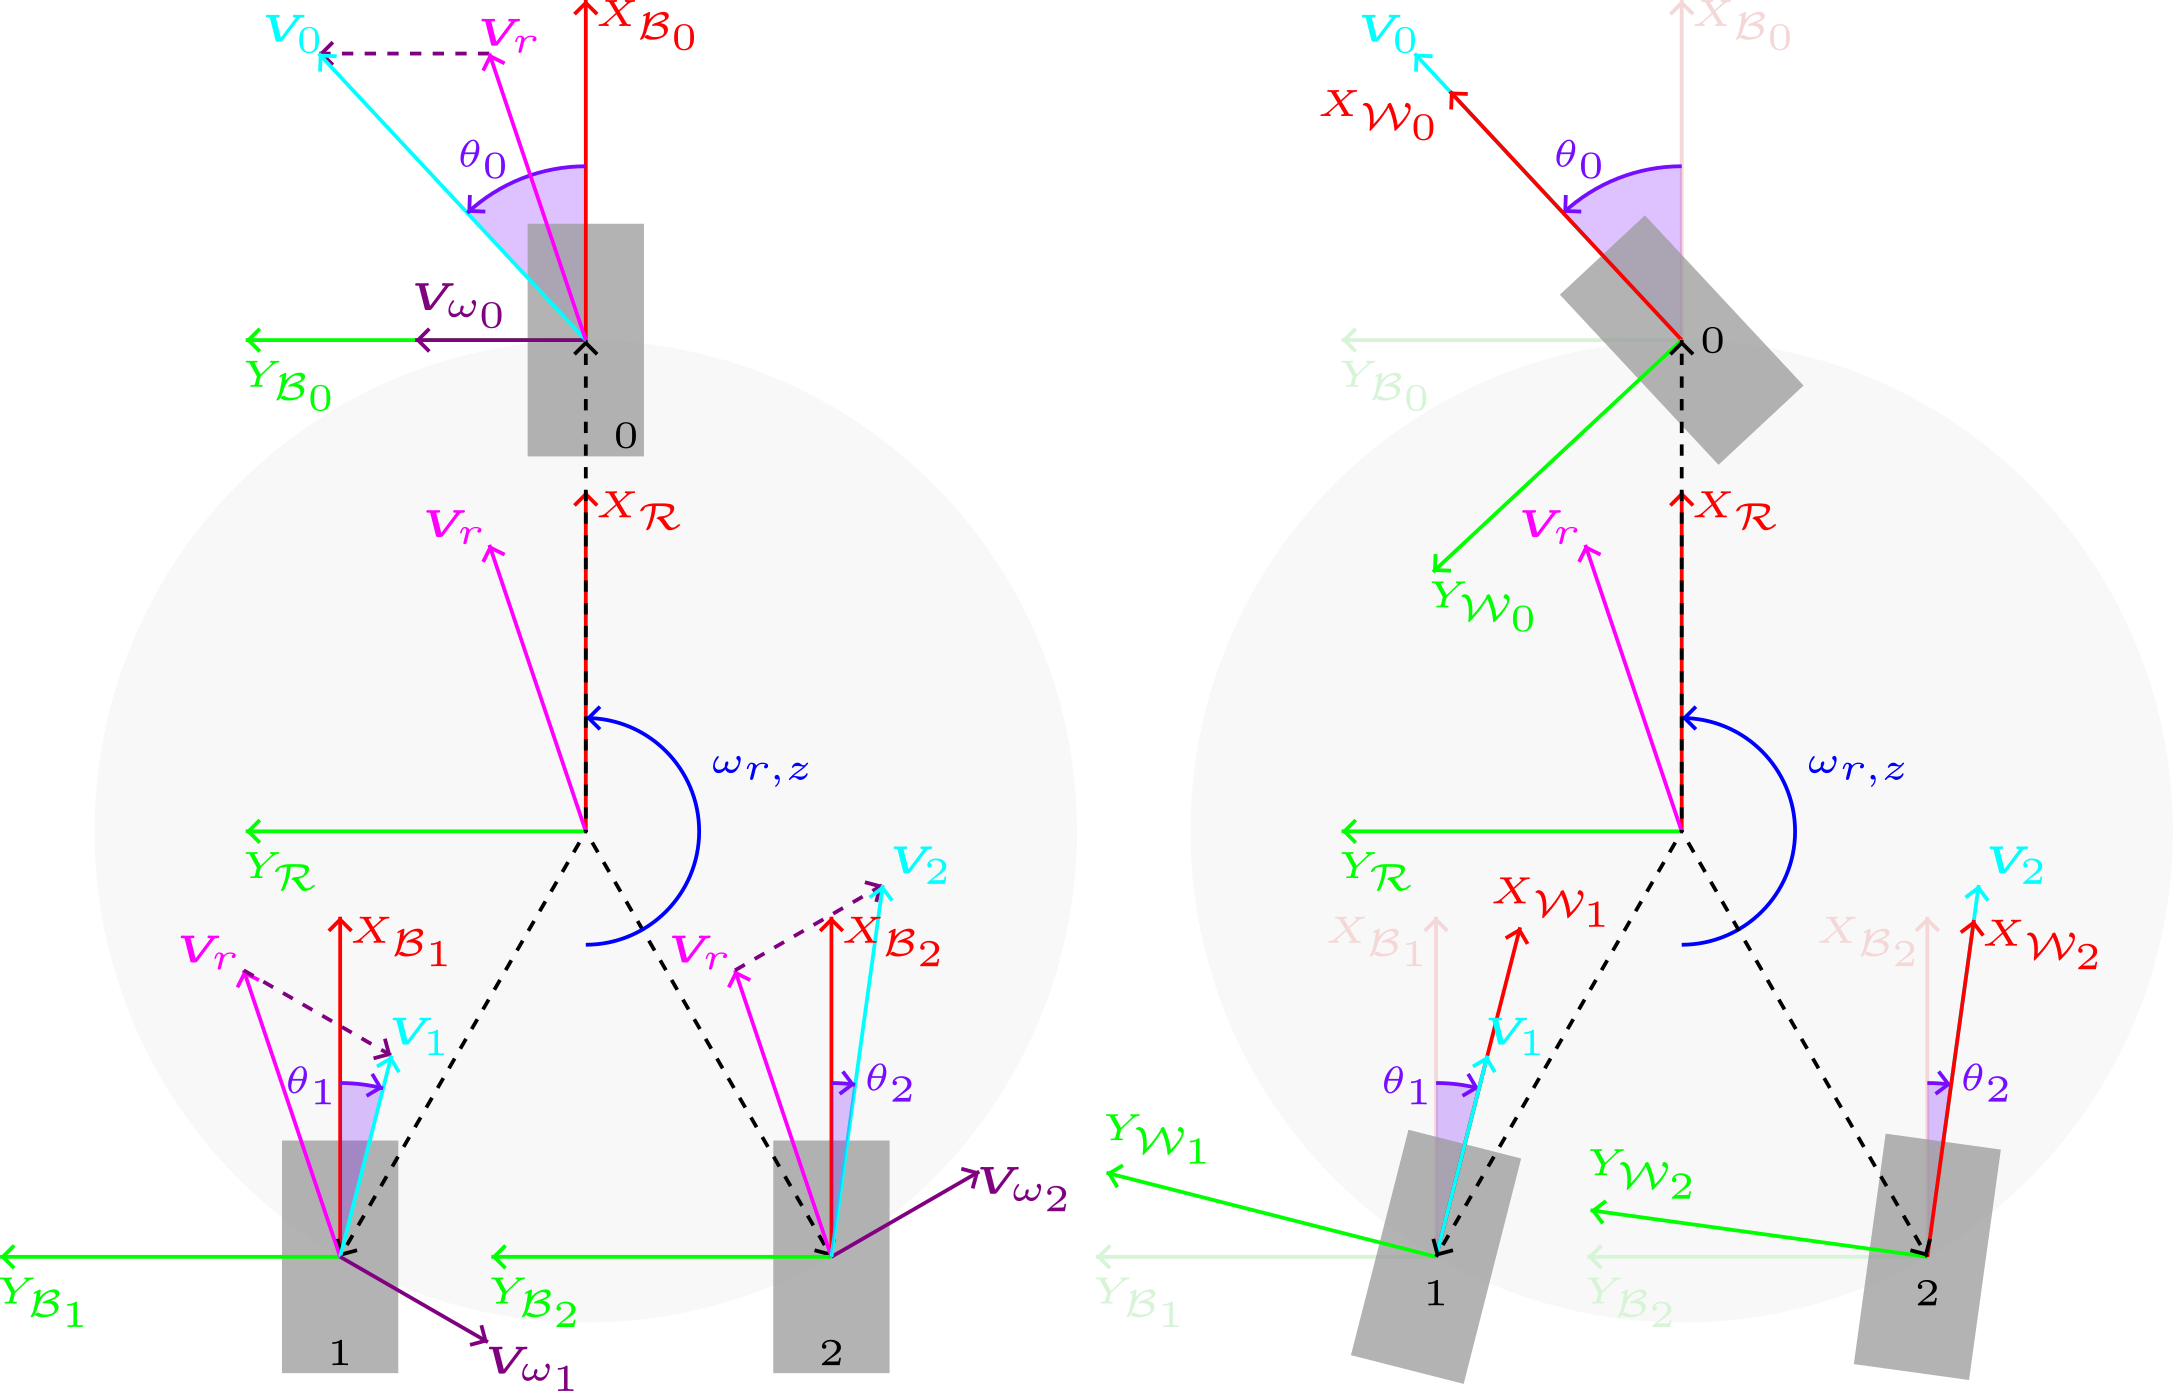
\includegraphics[width=1.0\linewidth]{images/three_swerve_drive_inverted_y_inverse_kinematics.png}
    \caption{Inverted-Y configuration. Left: Calculation of the velocity vector for each wheel, \(\vect{V}_i\). Right: Final orientation that each wheel must adopt (\(\theta_i\)) to align its rolling direction with the velocity vector \(\vect{V}_i\).}
    \label{fig2:tsd-inverted-y-inverse-kinematics}
\end{figure}

\begin{figure}[H]
    \centering
    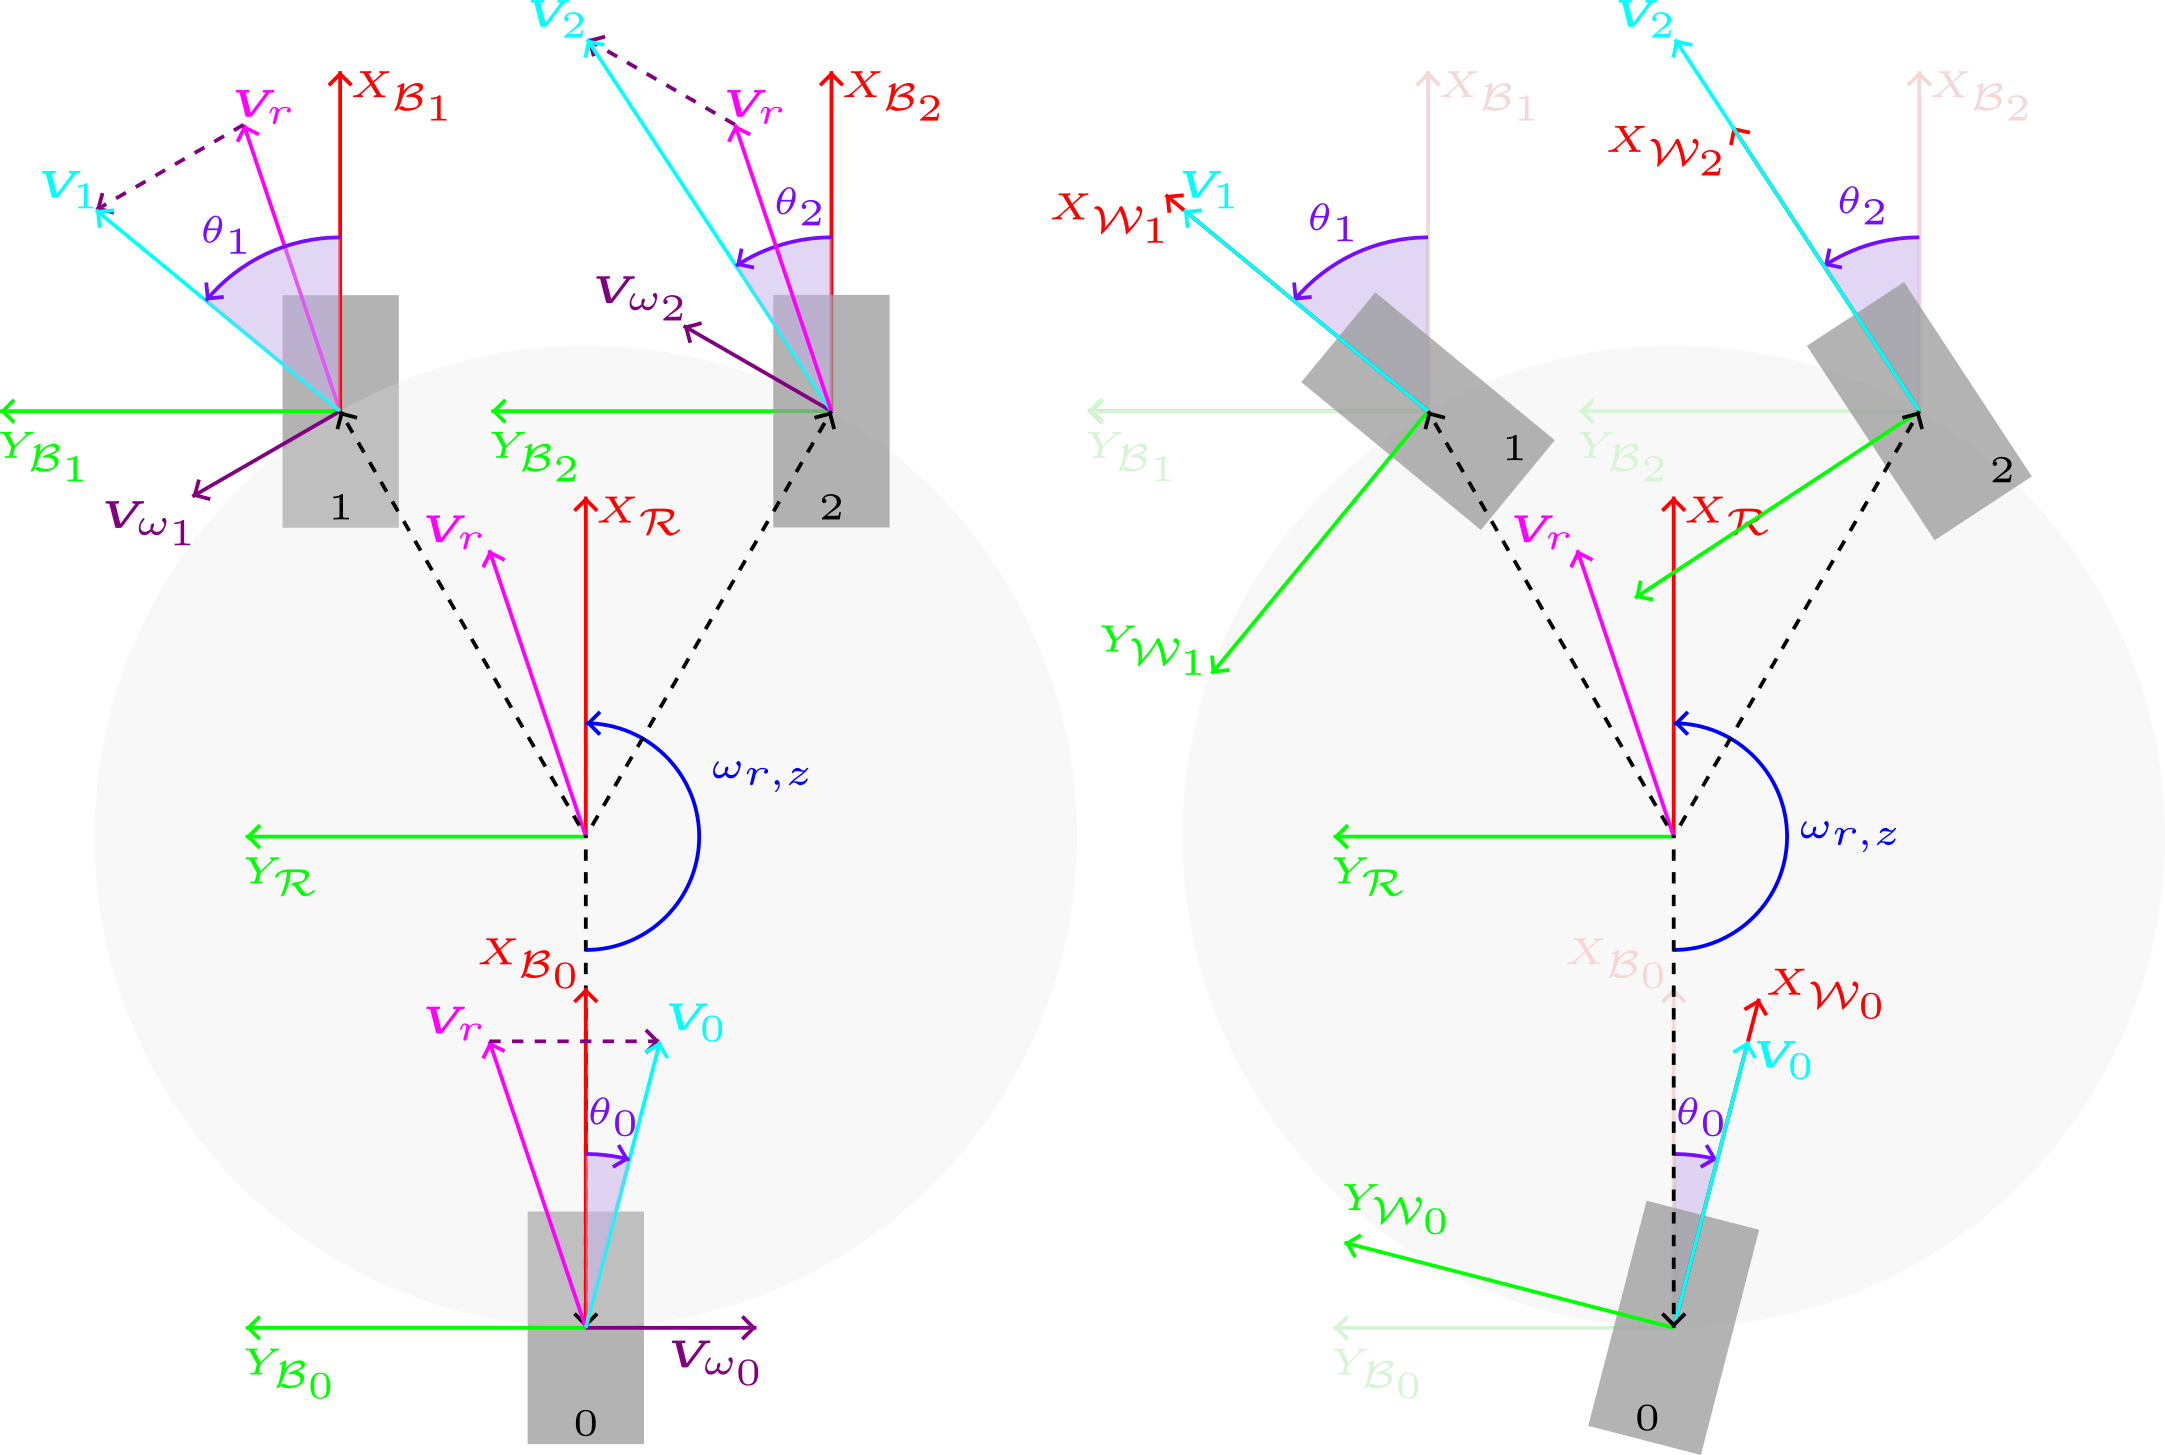
\includegraphics[width=1.0\linewidth]{images/three_swerve_drive_y_inverse_kinematics.png}
    \caption{Y configuration. Left: Calculation of the velocity vector for each wheel, \(\vect{V}_i\). Right: Final orientation that each wheel must adopt (\(\theta_i\)) to align its rolling direction with the velocity vector \(\vect{V}_i\).}
    \label{fig2:tsd-y-inverse-kinematics}
\end{figure}

\subsection{Forward kinematics of the three swerve}

Known the steering angle \(\theta_i\) and the angular velocity \(\omega_i\) of each wheel \(i\), the following steps are executed to calculate the forward kinematics of a robot with a three swerve drive base:

\begin{itemize}
    \item Calculate the vector \(\mathbf{b} = [{}^{\frameBZero}V_{0,x}, {}^{\frameBZero}V_{0,y}, \ldots, {}^{\frameBNMinusOne}V_{N-1,x}, {}^{\frameBNMinusOne}V_{N-1,y}]^{\trans}\).\\
          Where:
          \begin{equation}
              \begin{aligned}
                  {}^{\frameBi}V_{i,x} & = \|{}^{\frameBi}\vect{V}_i\| \cos\theta_i = v_{i\parallel}\cos\theta_i = r\omega_i\cos\theta_i \\
                  {}^{\frameBi}V_{i,y} & = \|{}^{\frameBi}\vect{V}_i\| \sin\theta_i = v_{i\parallel}\sin\theta_i = r\omega_i\sin\theta_i
              \end{aligned}
          \end{equation}
    \item Solve the linear system \(A\mathbf{x} = \mathbf{b}\) using the pseudoinverse of \(A\), \(A^+\), as explained in Section \ref{sec:general-considerations}, to obtain the chassis velocity \(\mathbf{x} = [{}^\frameR V_{r,x}, {}^\frameR V_{r,y}, \omega_{r,z}]^{\trans}\). Obviously, using the matrix \(A\) corresponding to the considered wheel configuration, inverted-Y or Y.
\end{itemize}

\section{Kinematics of a four swerve drive robot}

The base with four steerable active wheels (four swerve drive) is also an
omnidirectional locomotion system. As in the three swerve drive case, each
wheel can align its rolling direction with the velocity vector that appears at
its contact point. The chassis can therefore command the planar velocity
\({}^{\frameR}\vect{V}_r = [{}^{\frameR}V_{r,x}, {}^{\frameR}V_{r,y},
\omega_{r,z}]^{\trans}\), while each wheel independently selects its steering
angle and rolling speed.

All wheels are assumed to have the same radius \(r\). The position of wheel
\(i\) with respect to the robot frame \(\frameR\) is:

\begin{equation}
    \vect{d}_i = (x_i, y_i)
\end{equation}

As in the previous section, the base coordinate system of each wheel is chosen
so that:

\[
    \begin{aligned}
        \psi_i = \phi_i - \frac{\pi}{2} = 0 \quad          & \Longrightarrow \quad \phi_i = \frac{\pi}{2}             \\
        \phi_i = \alpha_i + \beta_i = \frac{\pi}{2}, \quad & \Longrightarrow \quad \beta_i = \frac{\pi}{2} - \alpha_i
    \end{aligned}
\]

Therefore:

\[
    {}^{\frameBi} R\left(\phi_i = \frac{\pi}{2}\right)_{\frameR} =
    \begin{bmatrix}
        1 & 0 \\
        0 & 1
    \end{bmatrix}
\]

The velocity of wheel \(i\), expressed in its base coordinate system, is:

\begin{equation}
    {}^{\frameBi}\vect{V}_i =
    \begin{bmatrix}
        {}^{\frameBi}V_{i,x} \\
        {}^{\frameBi}V_{i,y}
    \end{bmatrix}
    =
    \begin{bmatrix}
        {}^{\frameR}V_{r,x} - \omega_{r,z}y_i \\
        {}^{\frameR}V_{r,y} + \omega_{r,z}x_i
    \end{bmatrix}
\end{equation}

Stacking the four wheel velocity vectors gives the linear system
\(A\mathbf{x} = \mathbf{b}\), where
\(\mathbf{x} = [{}^{\frameR}V_{r,x}, {}^{\frameR}V_{r,y},
\omega_{r,z}]^{\trans}\) and:

\begin{equation}
    A =
    \begin{bmatrix}
        1 & 0 & -y_0           \\
        0 & 1 & \phantom{-}x_0 \\
        1 & 0 & -y_1           \\
        0 & 1 & \phantom{-}x_1 \\
        1 & 0 & -y_2           \\
        0 & 1 & \phantom{-}x_2 \\
        1 & 0 & -y_3           \\
        0 & 1 & \phantom{-}x_3
    \end{bmatrix}
\end{equation}

For a rectangular four swerve drive base, let \(a > 0\) be the distance from the
robot center to the front or rear wheel line, and let \(b > 0\) be the distance
from the robot center to the left or right wheel line. With the wheel order
front-left, front-right, rear-left, rear-right:

\[
    \begin{aligned}
        \vect{d}_0 & = (a, b)   &
        \vect{d}_1 & = (a, -b)  &
        \vect{d}_2 & = (-a, b)  &
        \vect{d}_3 & = (-a, -b)
    \end{aligned}
\]

and the matrix \(A\) becomes:

\begin{equation}
    A =
    \begin{bmatrix}
        1 & 0 & -b           \\
        0 & 1 & \phantom{-}a \\
        1 & 0 & \phantom{-}b \\
        0 & 1 & \phantom{-}a \\
        1 & 0 & -b           \\
        0 & 1 & -a           \\
        1 & 0 & \phantom{-}b \\
        0 & 1 & -a
    \end{bmatrix}
\end{equation}

\subsection{Inverse kinematics of the four swerve}

Given the chassis velocity vector \({}^{\frameR}\vect{V}_r\), the velocity of
each wheel is obtained from the corresponding two rows of \(A\):

\begin{equation}
    \begin{aligned}
        {}^{\frameBi}V_{i,x} & = {}^{\frameR}V_{r,x} - \omega_{r,z}y_i \\
        {}^{\frameBi}V_{i,y} & = {}^{\frameR}V_{r,y} + \omega_{r,z}x_i
    \end{aligned}
\end{equation}

The steering angle that wheel \(i\) must adopt is:

\begin{equation}
    \theta_i = \arctan2({}^{\frameBi}V_{i,y}, {}^{\frameBi}V_{i,x})
    \label{eq:fsd-inverse-kinematics-angle}
\end{equation}

The angular velocity of wheel \(i\) is:

\begin{equation}
    \omega_i =
    \frac{\sqrt{{}^{\frameBi}V_{i,x}^2 + {}^{\frameBi}V_{i,y}^2}}{r}
    \label{eq:fsd-inverse-kinematics-angular-speed}
\end{equation}

\subsection{Forward kinematics of the four swerve}

Known the steering angle \(\theta_i\) and angular velocity \(\omega_i\) of each
wheel, the velocity components measured in each wheel base frame are:

\begin{equation}
    \begin{aligned}
        {}^{\frameBi}V_{i,x} & = r\omega_i\cos\theta_i \\
        {}^{\frameBi}V_{i,y} & = r\omega_i\sin\theta_i
    \end{aligned}
\end{equation}

The vector \(\mathbf{b}\) is then built as:

\begin{equation}
    \mathbf{b} =
    \begin{bmatrix}
        {}^{\frameBZero}V_{0,x} \\
        {}^{\frameBZero}V_{0,y} \\
        {}^{\mathcal{B}_1}V_{1,x} \\
        {}^{\mathcal{B}_1}V_{1,y} \\
        {}^{\mathcal{B}_2}V_{2,x} \\
        {}^{\mathcal{B}_2}V_{2,y} \\
        {}^{\mathcal{B}_3}V_{3,x} \\
        {}^{\mathcal{B}_3}V_{3,y}
    \end{bmatrix}
\end{equation}

Since the four swerve drive provides eight scalar wheel velocity equations for
the three chassis velocity components, the system is overdetermined. The
chassis velocity is therefore obtained with the pseudoinverse of \(A\):

\begin{equation}
    \mathbf{x} = A^+\mathbf{b}
\end{equation}

where:

\begin{equation}
    \mathbf{x} =
    \begin{bmatrix}
        {}^{\frameR}V_{r,x} \\
        {}^{\frameR}V_{r,y} \\
        \omega_{r,z}
    \end{bmatrix}
\end{equation}

When all four wheel measurements are mutually consistent, the solution
reconstructs the commanded chassis velocity. When small inconsistencies appear
because of steering errors, encoder noise, wheel slip, or calibration errors,
the pseudoinverse gives the least-squares chassis velocity that best fits all
four wheel velocity vectors.

\end{document}
